%% =====================================================================
%%  Explainable SYN/UDP Flood Detection at the IoT Edge:
%%  A Lightweight Fuzzy Decision Tree for Transport-Layer Network Forensics
%%
%%  IEEE conference format (IEEEtran). Self-contained: every figure is drawn
%%  with TikZ/pgfplots, so the file compiles on its own (e.g. in Overleaf)
%%  without any external image files. Optional AI-generated illustrations
%%  can be swapped in where marked "OPTIONAL IMAGE" (see IMAGE_PROMPTS.md).
%% =====================================================================
\documentclass[conference]{IEEEtran}
\IEEEoverridecommandlockouts

\usepackage[T1]{fontenc}
\usepackage{cite}
\usepackage{amsmath,amssymb,amsfonts}
\usepackage{algorithm}
\usepackage{algpseudocode}
\usepackage{graphicx}
\usepackage{textcomp}
\usepackage{xcolor}
\usepackage{booktabs}
\usepackage{multirow}
\usepackage{array}
\usepackage{microtype}
\usepackage{url}
\usepackage{tikz}
\usetikzlibrary{arrows.meta,positioning,fit,backgrounds,calc,shapes.geometric,shapes.misc,decorations.pathreplacing}
\usepackage{pgfplots}
\pgfplotsset{compat=1.17}
\usepgfplotslibrary{groupplots}

% ---------------------------------------------------------------------
% Palette (colour-blind friendly) and helpers
% ---------------------------------------------------------------------
\definecolor{atk}{HTML}{C0392B}   % attack / block
\definecolor{nrm}{HTML}{2E8B57}   % normal / allow
\definecolor{sus}{HTML}{D4A017}   % suspicious / throttle
\definecolor{fz}{HTML}{1F6F8B}    % fuzzy layer
\definecolor{gr}{HTML}{5B6573}    % neutral
\definecolor{vio}{HTML}{6C4AB6}   % baselines
\definecolor{trn}{HTML}{3B7DD8}   % train split
\definecolor{tst}{HTML}{E67E22}   % test split

\newcommand{\yes}{\checkmark}
\newcommand{\no}{$\times$}
\newcommand{\partl}{$\sim$}
\newcommand{\fname}{\textsc{FuzzyForensIoT}}
\newcommand{\hd}[1]{\begin{tabular}[c]{@{}c@{}}#1\end{tabular}}

\tikzset{
  box/.style={draw=#1!75!black, fill=#1!10, rounded corners=2pt, align=center,
              font=\scriptsize, minimum height=0.95cm, text width=1.62cm, inner sep=2pt},
  arr/.style={-{Stealth[length=1.7mm]}, semithick, draw=black!70},
  darr/.style={-{Stealth[length=1.7mm]}, semithick, dashed, draw=black!60},
  lane/.style={draw=black!35, dashed, rounded corners=4pt, inner sep=5pt},
  tag/.style={font=\scriptsize\bfseries, text=black!75},
  fsmstate/.style={circle, draw=#1!75!black, fill=#1!15, thick, minimum size=1.35cm, align=center, font=\scriptsize\bfseries},
}

\algrenewcommand\algorithmicrequire{\textbf{Input:}}
\algrenewcommand\algorithmicensure{\textbf{Output:}}

\begin{document}

\title{Explainable SYN/UDP Flood Detection at the IoT Edge: A Lightweight Fuzzy Decision Tree for Transport-Layer Network Forensics}

\author{
\IEEEauthorblockN{Abhishek Anand}
\IEEEauthorblockA{\textit{Dept. of CSE}\\
\textit{Indian Institute of Information}\\
\textit{Technology Sri City}\\
Chittoor, Andhra Pradesh, India
% e-mail: add here
}
\and
\IEEEauthorblockN{Neha Agarwal}
\IEEEauthorblockA{\textit{Dept. of CSE}\\
\textit{Indian Institute of Information}\\
\textit{Technology Sri City}\\
Chittoor, Andhra Pradesh, India
% e-mail: add here
}
\and
\IEEEauthorblockN{Pavan Kumar B N}
\IEEEauthorblockA{\textit{Dept. of CSE}\\
\textit{Indian Institute of Information}\\
\textit{Technology Sri City}\\
Chittoor, Andhra Pradesh, India
% e-mail: add here
}
}

\maketitle

% =====================================================================
\begin{abstract}
Internet-of-Things (IoT) networks are a prime target of transport-layer denial-of-service floods, yet IoT network forensics is still largely manual: analysts read Wireshark I/O graphs and apply display filters to count SYN and SYN-ACK packets. Learning-based detectors automate this step but are usually too heavy for edge hardware and too opaque for an analyst who must justify blocking a host. This paper presents \fname{}, an explainable edge intrusion-detection and forensic-triage framework. It turns the transport-layer indicators that manual IoT forensics relies on (SYN/ACK imbalance, half-open connections, packet-rate bursts, source and port dispersion) into graded, human-readable verdicts. Twenty-two rolling-window features are mapped to 30 data-driven triangular membership grades and eight direction-gated expert rules. A cost-complexity-pruned decision tree is then trained only on this fuzzy space and fused with the rule evidence. The fused threat score drives a graduated ALLOW/THROTTLE/BLOCK response on a Raspberry Pi. We also contribute two evaluation-hygiene steps for packet-window datasets. Direction-aware relabeling showed that 49.1\% of weakly labelled attack packets were in fact the victim's own replies. A buffered chronological split removes the leakage caused by overlapping rolling windows, which otherwise inflates accuracy by about two points. On a 194,792-packet lab capture with a leakage-free hold-out of 38,747 packets, the deployed 89-node (9.1\,KB) fuzzy decision tree reaches 87.74\% accuracy and an F1-score of 0.456. It outperforms an identically trained plain decision tree (86.39\%, 0.438) and a $125\times$ larger deep multilayer perceptron (86.51\%, 0.440), and raises 583 fewer false alarms than the plain tree. Every verdict comes with IF-THEN evidence that can be placed directly in a forensic report.
\end{abstract}

\begin{IEEEkeywords}
IoT security, network forensics, SYN flood, UDP flood, fuzzy decision tree, explainable intrusion detection, edge computing, Raspberry Pi
\end{IEEEkeywords}

% =====================================================================
\section{Introduction}
\label{sec:intro}

The Internet of Things now spans smart homes, medical devices and industrial control. Tens of billions of connected objects exchange data over standard Internet protocols~\cite{naing2023}. Most of these devices have little memory, little CPU and rarely receive security updates. This makes them both easy victims and easy recruits for denial-of-service (DoS) campaigns. The Mirai botnet showed the scale of the problem by turning around 600,000 compromised IoT devices into record-breaking floods~\cite{antonakakis2017,kolias2017}.

Transport-layer floods remain the workhorse of such campaigns. A TCP SYN flood abuses the three-way handshake. It leaves the victim with a backlog of half-open connections until legitimate clients are refused~\cite{eddy2007,cert1996}. A UDP flood saturates bandwidth and CPU with datagrams, and the victim answers closed ports with ICMP \emph{destination unreachable} messages~\cite{khaing2020}. Naing \emph{et al.} report that over 90\% of DoS attacks exploit TCP, with SYN flooding the most common form~\cite{naing2023}.

IoT forensics is commonly organised into device-, network- and cloud-level investigations~\cite{stoyanova2020}. At the network level, the state of practice is manual. Naing \emph{et al.}~\cite{naing2023} investigated SYN and UDP floods against two smart-home devices by applying Wireshark filters such as \texttt{tcp.flags.syn==1 \&\& tcp.flags.ack==0}. They concluded that an attack had occurred because 5,636 SYN packets received only 225 SYN-ACK replies. Khaing \emph{et al.}~\cite{khaing2020} identified UDP floods from bursts of ICMP host-unreachable packets and UDP datagrams sent to port~80. Both studies identify useful forensic indicators, but a human must apply the filters, read the graphs and decide. The analysis is reactive, does not scale to continuous monitoring, and gives a binary judgement with no measure of confidence.

On the reasoning side, Ye~\cite{ye2022} argued that digital evidence is inherently ``specious'' (neither fully guilty nor fully innocent). Ye proposed fuzzy decision trees (FDTs) built with Fuzzy-ID3 as a reasoning engine for proactive network forensics, where every root-to-leaf path becomes a fuzzy rule that a court can read. However, that work is conceptual. No membership functions are defined for network metrics, no dataset is used and no accuracy is reported.

At the edge, a detector must meet four requirements at once. It must be \emph{lightweight} (kilobytes, microseconds), \emph{accurate}, \emph{explainable}, and \emph{forensically sound} (it must attribute evidence to the attacker rather than the victim). Crisp thresholds fail in the grey zone where legitimate congestion and low-rate floods look alike. Deep models detect well~\cite{doshi2018,meidan2018}, but they consume megabytes and behave as black boxes~\cite{adadi2018}. Classical rule-based systems are interpretable but rigid and sensitive to hand-chosen constants~\cite{bridges2000}.

This paper closes the gap between manual transport-layer forensics~\cite{naing2023,khaing2020} and fuzzy forensic reasoning~\cite{ye2022}. Our contributions are:
\begin{enumerate}
  \item \textbf{\fname{}}, an end-to-end framework that turns raw IoT packet streams into graded flood verdicts using a fuzzy rule layer and a lightweight decision tree, together with human-readable evidence.
  \item A \textbf{direction-gated fuzzy rule base} with \textbf{data-driven membership placement}, which needs no hand-tuned constants, plus a rule--tree fusion score that drives a graduated response.
  \item \textbf{Evaluation hygiene for packet-window data}. Direction-aware relabeling corrects 49.1\% of weak attack labels. A buffered chronological split removes rolling-window leakage that otherwise inflates baseline accuracy by 2.06 points.
  \item A \textbf{controlled comparison} under one shared training protocol. The 9.1\,KB fuzzy tree beats an identically trained plain tree and a 1.14\,MB deep MLP on accuracy, precision and F1. Ablations isolate the contributions of the rules, the tree and the fusion step.
  \item A \textbf{Raspberry Pi deployment} with live capture, ALLOW/THROTTLE/BLOCK mitigation with time-to-live (TTL) auto-release, management safety rails, a forensic event log and an explanation dashboard.
\end{enumerate}

Section~\ref{sec:related} reviews related work. Section~\ref{sec:problem} formalises the problem. Section~\ref{sec:data} describes how the dataset was generated and conditioned. Section~\ref{sec:method} presents the fuzzy reasoning pipeline, and Section~\ref{sec:edge} the edge deployment. Sections~\ref{sec:setup} and~\ref{sec:results} report the experiments. Section~\ref{sec:limits} discusses limitations, and Section~\ref{sec:conclusion} concludes.

% ---------------------------------------------------------------------
% FIGURE 1 : overall architecture
% ---------------------------------------------------------------------
\begin{figure*}[t]
\centering
% OPTIONAL IMAGE: replace this TikZ block with
% \includegraphics[width=\textwidth]{figures/architecture.png}
\resizebox{\textwidth}{!}{%
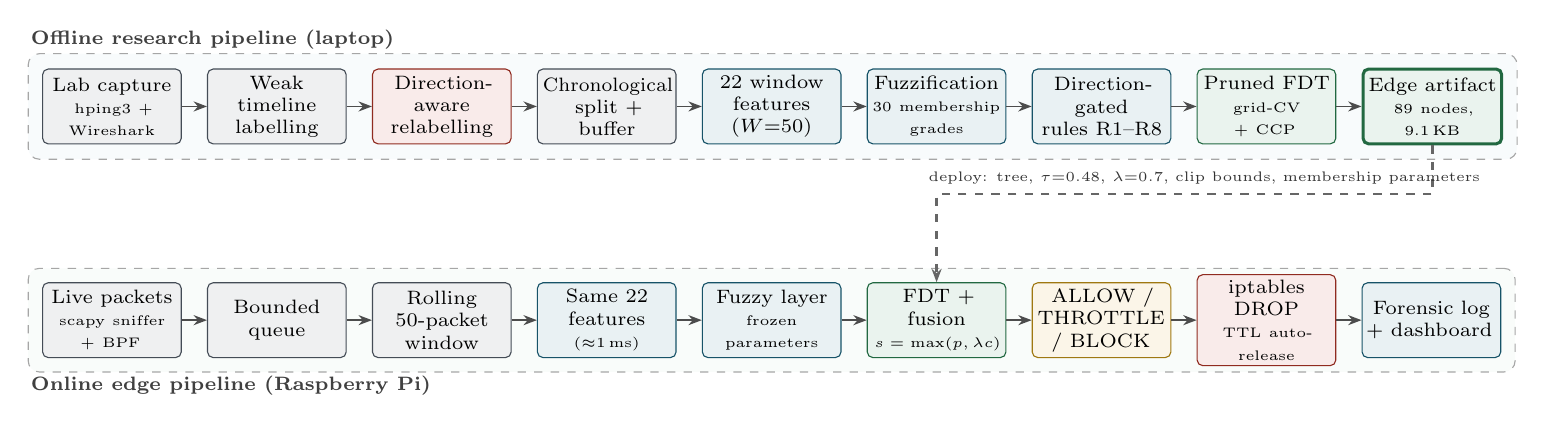
\begin{tikzpicture}[node distance=0.32cm]
  % ---- offline lane
  \node[box=gr] (t1) {Lab capture\\{\tiny hping3 + Wireshark}};
  \node[box=gr,  right=of t1] (t2) {Weak timeline\\labelling};
  \node[box=atk, right=of t2] (t3) {Direction-aware\\relabelling};
  \node[box=gr,  right=of t3] (t4) {Chronological\\split + buffer};
  \node[box=fz,  right=of t4] (t5) {22 window\\features ($W{=}50$)};
  \node[box=fz,  right=of t5] (t6) {Fuzzification\\{\tiny 30 membership grades}};
  \node[box=fz,  right=of t6] (t7) {Direction-gated\\rules R1--R8};
  \node[box=nrm, right=of t7] (t8) {Pruned FDT\\{\tiny grid-CV + CCP}};
  \node[box=nrm, right=of t8, line width=1.1pt] (t9) {Edge artifact\\{\tiny 89 nodes, 9.1\,KB}};
  \foreach \a/\b in {t1/t2,t2/t3,t3/t4,t4/t5,t5/t6,t6/t7,t7/t8,t8/t9}
     \draw[arr] (\a) -- (\b);
  % ---- online lane
  \node[box=gr,  below=1.75cm of t1] (b1) {Live packets\\{\tiny scapy sniffer + BPF}};
  \node[box=gr,  right=of b1] (b2) {Bounded\\queue};
  \node[box=gr,  right=of b2] (b3) {Rolling\\50-packet window};
  \node[box=fz,  right=of b3] (b4) {Same 22\\features {\tiny($\approx$1\,ms)}};
  \node[box=fz,  right=of b4] (b5) {Fuzzy layer\\{\tiny frozen parameters}};
  \node[box=nrm, right=of b5] (b6) {FDT + fusion\\{\tiny $s=\max(p,\lambda c)$}};
  \node[box=sus, right=of b6] (b7) {ALLOW /\\THROTTLE / BLOCK};
  \node[box=atk, right=of b7] (b8) {iptables DROP\\{\tiny TTL auto-release}};
  \node[box=fz,  right=of b8] (b9) {Forensic log\\+ dashboard};
  \foreach \a/\b in {b1/b2,b2/b3,b3/b4,b4/b5,b5/b6,b6/b7,b7/b8,b8/b9}
     \draw[arr] (\a) -- (\b);
  % ---- deployment link
  \draw[darr, line width=0.9pt] (t9.south) -- ++(0,-0.62) -| (b6.north)
     node[pos=0.23, above, font=\tiny, text=black!80] {deploy: tree, $\tau{=}0.48$, $\lambda{=}0.7$, clip bounds, membership parameters};
  % ---- lanes
  \begin{scope}[on background layer]
    \node[lane, fill=fz!3, fit=(t1)(t9),
          label={[tag, anchor=south west, inner sep=1pt]north west:Offline research pipeline (laptop)}] {};
    \node[lane, fill=nrm!3, fit=(b1)(b9),
          label={[tag, anchor=north west, inner sep=1pt]south west:Online edge pipeline (Raspberry Pi)}] {};
  \end{scope}
\end{tikzpicture}}
\caption{Overview of \fname{}. The offline pipeline conditions the capture, builds the fuzzy feature space and trains a pruned fuzzy decision tree. The edge pipeline reproduces the same feature and fuzzy transformations with frozen parameters, scores every 50-packet window and applies a graduated, reversible response with logged evidence.}
\label{fig:arch}
\end{figure*}

% =====================================================================
\section{Background and Related Work}
\label{sec:related}

\subsection{Transport-Layer Flooding Attacks}
In a legitimate TCP handshake the client sends SYN, the server answers SYN-ACK and allocates state, and the client completes with ACK (Fig.~\ref{fig:handshake}a). A SYN flood sends SYNs, often from spoofed addresses, and never completes the handshake. Each SYN-ACK is therefore sent into the void and the victim's backlog of half-open connections fills up (Fig.~\ref{fig:handshake}b)~\cite{eddy2007,cert1996}. The forensic signatures are a large SYN-to-SYN-ACK imbalance, a growing number of half-open connections, short SYN inter-arrival times and abnormal TCP fields. Naing \emph{et al.} observed flood SYNs with zero payload and a window size of 256~\cite{naing2023}. A UDP flood sprays datagrams at random or fixed ports. Closed ports trigger ICMP destination-unreachable replies, and UDP traffic towards TCP-only service ports (e.g., port~80) is itself anomalous~\cite{khaing2020}.

% ---------------------------------------------------------------------
% FIGURE 2 : handshake vs SYN flood
% ---------------------------------------------------------------------
\begin{figure}[t]
\centering
\resizebox{\columnwidth}{!}{%
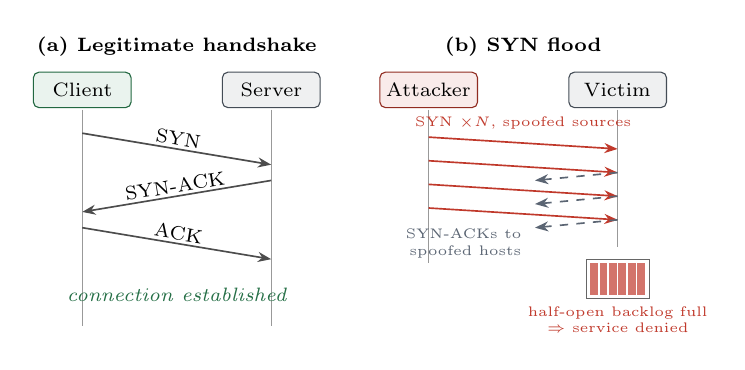
\begin{tikzpicture}[font=\scriptsize]
  % (a) legitimate handshake
  \node[font=\scriptsize\bfseries] at (1.2,0.55) {(a) Legitimate handshake};
  \node[box=nrm, text width=1.1cm, minimum height=0.45cm] (c) at (0,0) {Client};
  \node[box=gr,  text width=1.1cm, minimum height=0.45cm] (s) at (2.4,0) {Server};
  \draw[black!40] (0,-0.25) -- (0,-3.0);
  \draw[black!40] (2.4,-0.25) -- (2.4,-3.0);
  \draw[arr] (0,-0.55) -- node[above, sloped, inner sep=1pt] {SYN} (2.4,-0.95);
  \draw[arr] (2.4,-1.15) -- node[above, sloped, inner sep=1pt] {SYN-ACK} (0,-1.55);
  \draw[arr] (0,-1.75) -- node[above, sloped, inner sep=1pt] {ACK} (2.4,-2.15);
  \node[text=nrm!80!black, font=\scriptsize\itshape] at (1.2,-2.6) {connection established};
  % (b) SYN flood
  \node[font=\scriptsize\bfseries] at (5.6,0.55) {(b) SYN flood};
  \node[box=atk, text width=1.1cm, minimum height=0.45cm] (a) at (4.4,0) {Attacker};
  \node[box=gr,  text width=1.1cm, minimum height=0.45cm] (v) at (6.8,0) {Victim};
  \draw[black!40] (4.4,-0.25) -- (4.4,-2.2);
  \draw[black!40] (6.8,-0.25) -- (6.8,-2.0);
  \node[text=atk, font=\tiny] at (5.6,-0.42) {SYN $\times N$, spoofed sources};
  \foreach \y in {-0.6,-0.9,-1.2,-1.5}
     \draw[arr, draw=atk] (4.4,\y) -- (6.8,\y-0.15);
  \foreach \y in {-1.05,-1.35,-1.65}
     \draw[darr, draw=gr] (6.8,\y) -- (5.75,\y-0.1);
  \node[text=gr, font=\tiny, align=right, anchor=east] at (5.7,-1.95) {SYN-ACKs to\\spoofed hosts};
  % backlog
  \foreach \i in {0,...,5}
     \fill[atk!70] (6.45+\i*0.12,-2.2) rectangle ++(0.1,-0.4);
  \draw[black!60] (6.4,-2.15) rectangle (7.2,-2.65);
  \node[text=atk, font=\tiny, align=center] at (6.8,-2.92) {half-open backlog full\\$\Rightarrow$ service denied};
\end{tikzpicture}}
\caption{(a) A legitimate TCP handshake. (b) A SYN flood: unanswered SYN-ACKs leave half-open entries that exhaust the victim's backlog, producing the SYN/SYN-ACK imbalance observed manually in~\cite{naing2023}.}
\label{fig:handshake}
\end{figure}

\subsection{IoT Network Forensics}
Stoyanova \emph{et al.}~\cite{stoyanova2020} survey IoT forensics and highlight open problems in data heterogeneity, evidence preservation and legal admissibility. Network forensics follows a process model of preparation, detection, incident response, collection, preservation, examination, analysis, investigation and presentation~\cite{naing2023}. The two transport-layer studies that motivate this work~\cite{naing2023,khaing2020} carry out the detection and analysis stages by hand in Wireshark. Naing \emph{et al.} analysed a capture of more than 1\,GB (187,060 records) from an SKT NUGU speaker and an EZVIZ camera. They identified SYN floods from the SYN versus SYN-ACK counts, I/O-graph spikes, anomalous packet-length bins (40--2,599 bytes), and out-of-order and retransmitted segments. Khaing \emph{et al.} attributed UDP floods to four attacker addresses by filtering ICMP host-unreachable packets and UDP traffic to port~80. Koroniotis \emph{et al.} released Bot-IoT specifically for network-forensic analytics~\cite{koroniotis2019}. None of these works produces automated, confidence-graded verdicts.

\subsection{Fuzzy Logic and Fuzzy Decision Trees}
Fuzzy sets~\cite{zadeh1965} replace the crisp 0/1 indicator with a membership degree $\mu\in[0,1]$. This lets a value such as a SYN rate be ``somewhat high'' and ``somewhat medium'' at the same time. Decision-tree induction (ID3~\cite{quinlan1986}, CART~\cite{breiman1984}) recursively partitions data by an impurity criterion. Each root-to-leaf path is a conjunctive rule. Fuzzy-ID3~\cite{yuan1995} and related FDT methods~\cite{janikow1998} combine both ideas: attributes are fuzzified and a fuzzy entropy guides the splits. Ye~\cite{ye2022} applied this reasoning to network forensics. That work describes a four-step FDT construction (fuzzify the attributes, create the root, choose the best fuzzy split, recurse), extracts one rule per path, and argues for proactive rather than event-driven evidence collection. It contains no experiments.

\subsection{Machine-Learning and Fuzzy IDS for IoT DDoS}
Doshi \emph{et al.}~\cite{doshi2018} showed that lightweight packet and flow features separate consumer-IoT DDoS traffic well. N-BaIoT~\cite{meidan2018} uses per-device deep autoencoders. Dimolianis \emph{et al.}~\cite{dimolianis2021} classify SYN floods with machine learning and mitigate them with programmable data-plane filters. Fuzzy approaches include an FIS-based DDoS IDS evaluated on IoT-23~\cite{hoang2022}, a hybrid ML--fuzzy-cognitive-map detector aimed at resource-constrained devices~\cite{keshavamurthy2024}, and FLSec-RPL, a fuzzy IDS with a blocking stage for RPL routing attacks~\cite{kim2024}. Large IoT attack benchmarks such as CICIoT2023~\cite{neto2023} have made these comparisons more systematic.

\subsection{Research Gap}
Table~\ref{tab:related} positions this work. The forensic studies~\cite{naing2023,khaing2020} provide validated transport-layer indicators but no automation. The FDT forensics model~\cite{ye2022} provides the reasoning paradigm but no implementation. Fuzzy and ML IDS works automate detection but do not combine KB-scale edge deployment, per-verdict forensic explanations and attacker-direction attribution in a single system. To our knowledge, no prior system defines membership functions for IoT transport-layer flood metrics and trains an FDT-style model on real IoT packet captures to emit confidence-graded, court-readable rules.

\begin{table*}[t]
\centering
\caption{Positioning against the base papers and related IoT DDoS detectors (\yes{} = provided, \partl{} = partial or claimed, \no{} = absent, -- = not reported)}
\label{tab:related}
\footnotesize
\renewcommand{\arraystretch}{1.12}
\resizebox{\textwidth}{!}{%
\begin{tabular}{@{}l l c c c c c c@{}}
\toprule
\textbf{Work} & \textbf{Target attack} & \textbf{Automated} & \hd{\textbf{Fuzzy}\\\textbf{reasoning}} & \hd{\textbf{Empirical}\\\textbf{data}} & \hd{\textbf{Edge-}\\\textbf{deployable}} & \hd{\textbf{Per-verdict}\\\textbf{explanation}} & \textbf{Mitigation} \\
\midrule
Naing \emph{et al.}~\cite{naing2023} (base) & TCP-SYN, UDP flood & \no & \no & \yes & \no & \partl{} (analyst) & \no \\
Khaing \emph{et al.}~\cite{khaing2020} (base) & UDP flood & \no & \no & \yes & \no & \partl{} (analyst) & \no \\
Ye~\cite{ye2022} (base) & Generic intrusion & \partl{} (conceptual) & \yes & \no & \no & \yes{} (conceptual) & \no \\
Dimolianis \emph{et al.}~\cite{dimolianis2021} & TCP-SYN flood & \yes & \no & \yes & \yes{} (data plane) & -- & \yes \\
Hoang \emph{et al.}~\cite{hoang2022} & DDoS (IoT-23) & \yes & \yes{} (FIS) & \yes & \partl & \partl & -- \\
Keshavamurthy \& Kulkarni~\cite{keshavamurthy2024} & DDoS & \yes & \yes{} (FCM) & \yes & \partl & \partl & -- \\
Kim \emph{et al.}~\cite{kim2024} & RPL DIO suppression & \yes & \yes & \partl{} (simulation) & \partl & \partl & \yes \\
\midrule
\textbf{\fname{} (this work)} & \textbf{TCP-SYN, UDP flood} & \yes & \yes{} (rules + FDT) & \yes & \yes{} (Raspberry Pi) & \yes{} (rules + path) & \yes{} (graduated) \\
\bottomrule
\end{tabular}}
\end{table*}

% =====================================================================
\section{Problem Formulation and Design Goals}
\label{sec:problem}

Let $\mathcal{P}=\langle p_1,p_2,\dots\rangle$ be the packet stream observed at an IoT edge node. Each packet $p_i$ has a timestamp $t_i$, source and destination addresses and ports, a protocol, a length $\ell_i$ and TCP flags. For every packet we form the backward-looking window
\begin{equation}
  \mathcal{W}_i=\langle p_{i-W+1},\dots,p_i\rangle,\qquad W=50,
  \label{eq:window}
\end{equation}
and a feature vector $\mathbf{x}_i=\phi(\mathcal{W}_i)\in\mathbb{R}^{22}$. The label is $y_i=1$ if and only if $p_i$ flows from an attacker to the victim during an attack phase. The victim's replies are deliberately labelled $0$ (Section~\ref{sec:relabel}). We seek a decision function
\begin{equation}
  f:\mathbf{x}_i\mapsto(\hat{y}_i,\;s_i,\;\mathcal{E}_i),
\end{equation}
which returns a verdict $\hat{y}_i$, a threat score $s_i\in[0,1]$ and an explanation $\mathcal{E}_i$ made of named rule activations and the decision path. The design goals are:
\begin{itemize}
  \item \textbf{G1 Lightweight:} kilobyte-scale model with microsecond inference on a single CPU core.
  \item \textbf{G2 Accurate:} at least as accurate as a deep baseline under leakage-free evaluation.
  \item \textbf{G3 Explainable:} every verdict maps to named forensic indicators.
  \item \textbf{G4 Forensically sound:} evidence is attributed to attacker-direction traffic, and the response is graded, reversible and logged.
\end{itemize}

% =====================================================================
\section{Dataset Generation and Conditioning}
\label{sec:data}

\subsection{Testbed and Attack Generation}
Fig.~\ref{fig:testbed} shows the testbed. A Raspberry Pi acts as the target IoT edge node on an isolated lab Wi-Fi network. An attacker laptop runs \texttt{hping3}~\cite{hping3} with a scripted attack cycle: a 20\,s SYN flood to port~80 (\texttt{-S -p 80 -i u2000 -{}-rand-source}, nominally 500\,pps), 10\,s of silence, and a 20\,s UDP flood to port~53 (\texttt{-2 -p 53}). Each phase boundary is written with its wall-clock timestamp to \texttt{labels\_map.txt}. Traffic is captured with Wireshark/tcpdump and exported to CSV with the fields time, source, destination, protocol, length and info. Ordinary devices on the same network contribute realistic background traffic (TCP, QUIC, DNS, mDNS, ARP, ICMPv6 and TLS). Table~\ref{tab:dataset} summarises the capture.

% ---------------------------------------------------------------------
% FIGURE 3 : testbed
% ---------------------------------------------------------------------
\begin{figure}[t]
\centering
\resizebox{\columnwidth}{!}{%
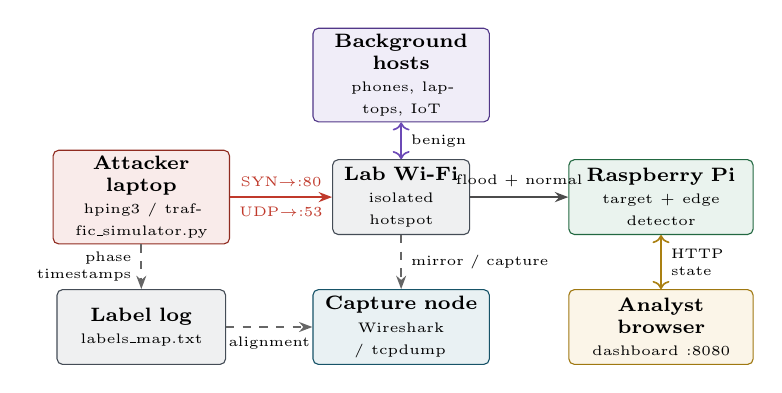
\begin{tikzpicture}[font=\scriptsize]
  \node[box=atk, text width=2.1cm] (att) at (0,0) {\textbf{Attacker laptop}\\{\tiny hping3 / traffic\_simulator.py}};
  \node[box=gr,  text width=1.6cm] (ap) at (3.3,0) {\textbf{Lab Wi-Fi}\\{\tiny isolated hotspot}};
  \node[box=nrm, text width=2.2cm] (pi) at (6.6,0) {\textbf{Raspberry Pi}\\{\tiny target + edge detector}};
  \node[box=vio, text width=2.1cm] (bg) at (3.3,1.55) {\textbf{Background hosts}\\{\tiny phones, laptops, IoT}};
  \node[box=fz,  text width=2.1cm] (cap) at (3.3,-1.65) {\textbf{Capture node}\\{\tiny Wireshark / tcpdump}};
  \node[box=gr,  text width=2.0cm] (lab) at (0,-1.65) {\textbf{Label log}\\{\tiny labels\_map.txt}};
  \node[box=sus, text width=2.2cm] (an) at (6.6,-1.65) {\textbf{Analyst browser}\\{\tiny dashboard :8080}};
  \draw[arr, draw=atk, line width=0.9pt] (att) -- node[above, font=\tiny, text=atk] {SYN$\to$:80} node[below, font=\tiny, text=atk] {UDP$\to$:53} (ap);
  \draw[arr, line width=0.9pt] (ap) -- node[above, font=\tiny] {flood + normal} (pi);
  \draw[arr, <->, draw=vio] (bg) -- node[right, font=\tiny] {benign} (ap);
  \draw[darr] (ap) -- node[right, font=\tiny] {mirror / capture} (cap);
  \draw[darr] (att) -- node[left, font=\tiny, align=right] {phase\\timestamps} (lab);
  \draw[darr] (lab) -- node[below, font=\tiny] {alignment} (cap);
  \draw[arr, <->, draw=sus!80!black] (pi) -- node[right, font=\tiny, align=left] {HTTP\\state} (an);
\end{tikzpicture}}
\caption{Lab testbed. Floods and benign traffic reach the Raspberry Pi through an isolated Wi-Fi network. The capture is aligned with the attack-phase timestamps logged by the generator, and the Pi serves the live dashboard.}
\label{fig:testbed}
\end{figure}

\begin{table}[t]
\centering
\caption{Lab capture statistics}
\label{tab:dataset}
\footnotesize
\renewcommand{\arraystretch}{1.08}
\setlength{\tabcolsep}{4pt}
\begin{tabular}{@{}l r@{}}
\toprule
\textbf{Property} & \textbf{Value} \\
\midrule
Packets captured & 194,792 \\
Duration & 2,283\,s ($\approx$38\,min) \\
TCP / UDP / QUIC / ICMP share & 73.8 / 16.5 / 5.2 / 2.6\% \\
SYN-flood phase (weak label) & 20.1\,s, 20,572 pkts, 1,025\,pps \\
Second flood phase (weak label) & 20.0\,s, 8,371 pkts, 419\,pps \\
Weakly labelled attack packets & 28,943 (14.86\%) \\
Victim replies relabelled normal & 14,208 (49.1\%) \\
Unrelated background relabelled & 215 \\
\textbf{Final attack / normal packets} & \textbf{14,520 (7.45\%) / 180,272} \\
Train / test / buffer (dropped) & 155,835 / 38,747 / 210 \\
Attack ratio train / test & 7.38\% / 7.64\% \\
\bottomrule
\end{tabular}
\end{table}

\subsection{Weak Timeline Labelling}
The generator logs phase boundaries in wall-clock time, while the capture uses relative timestamps. The labeller therefore aligns the two timelines. It uses the capture's start epoch when available, and otherwise searches for the offset (on a 0.1\,s grid) that maximises the contrast between the packet rates inside and outside the attack intervals. Every packet inside an attack interval receives the label $1$. This produces 28,943 weakly labelled attack packets.

\subsection{Direction-Aware Relabelling}
\label{sec:relabel}
Window-based labels are cheap but noisy. During a SYN flood, a large share of the packets inside the attack window are the \emph{victim's own} SYN-ACK and RST replies. A model trained to call these ``attack'' learns to flag the victim, which caps its recall and, in deployment, triggers alarms on the edge node's own traffic. Algorithm~\ref{alg:relabel} infers the victim of each attack window and relabels its replies and any unrelated background chatter as normal. This step reverted 14,208 victim replies (49.1\%) and 215 background packets, leaving 14,520 attacker-to-victim packets. In our development experiments, removing this label noise raised the ROC-AUC from about 0.79 to about 0.90.

\begin{algorithm}[t]
\caption{Direction-aware relabelling}
\label{alg:relabel}
\begin{algorithmic}[1]
\Require weakly labelled packets; contiguous attack windows $\{\mathcal{I}_j\}$
\Ensure corrected labels $y$
\For{each attack window $\mathcal{I}_j$}
  \State $v\gets$ mode of $\mathrm{dst}(p)$ over SYN-only packets in $\mathcal{I}_j$
  \If{no SYN-only packets} \State $v\gets$ mode of $\mathrm{src}(p)$ over RST packets
  \EndIf
  \If{still undefined} \State $v\gets$ mode of $\mathrm{dst}(p)$ over TCP/UDP packets
  \EndIf
  \For{each $p\in\mathcal{I}_j$}
    \If{$\mathrm{src}(p)=v$} \State $y(p)\gets 0$ \Comment{victim reply}
    \ElsIf{$\mathrm{proto}(p)\notin\{\mathrm{TCP,UDP,QUIC}\}$} \State $y(p)\gets 0$ \Comment{background}
    \ElsIf{$\mathrm{proto}(p)=\mathrm{QUIC}\wedge \mathrm{dst}(p)\neq v$} \State $y(p)\gets 0$
    \EndIf
  \EndFor
\EndFor
\end{algorithmic}
\end{algorithm}

\subsection{Leakage-Free Chronological Split}
All features are rolling-window statistics, so neighbouring rows overlap almost completely:
\begin{equation}
  |\mathcal{W}_i\cap\mathcal{W}_{i+k}| = W-k \quad (0\le k<W).
\end{equation}
A random row split therefore places near-duplicates of each test row in the training set. With such a split, an unpruned plain tree reached 88.45\% accuracy, against 86.39\% under the honest protocol (Section~\ref{sec:ablation}). We instead split \emph{each contiguous traffic segment} chronologically. The first 80\% of every segment is used for training, the last 20\% is held out, and the 50 packets at the boundary are dropped (Fig.~\ref{fig:conditioning}b). Because the features look only backwards, no training window can contain a held-out packet.

% ---------------------------------------------------------------------
% FIGURE 4 : data conditioning
% ---------------------------------------------------------------------
\begin{figure}[t]
\centering
\resizebox{\columnwidth}{!}{%
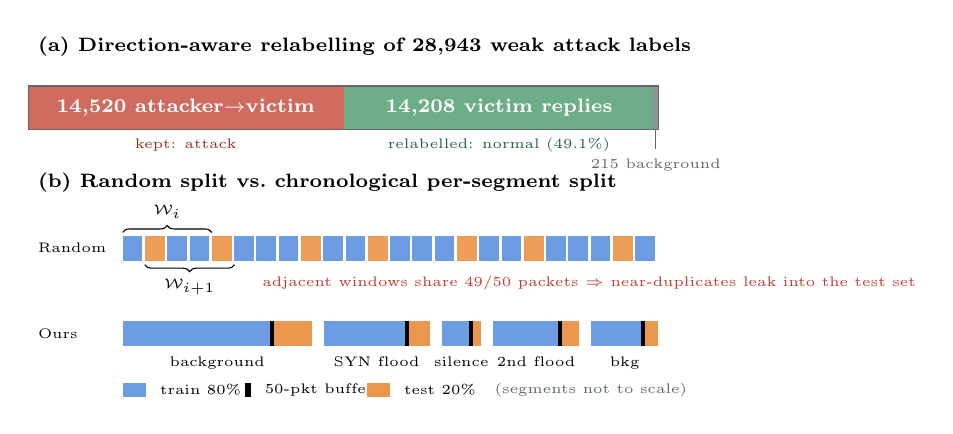
\begin{tikzpicture}[font=\scriptsize]
  % (a) relabelling bar (total width 8 cm  <-> 28,943 packets)
  \node[font=\scriptsize\bfseries, anchor=west] at (0,1.05) {(a) Direction-aware relabelling of 28,943 weak attack labels};
  \fill[atk!75]  (0,0) rectangle (4.013,0.55);
  \fill[nrm!70]  (4.013,0) rectangle (7.940,0.55);
  \fill[gr!70]   (7.940,0) rectangle (8.0,0.55);
  \draw[black!60] (0,0) rectangle (8,0.55);
  \node[text=white, font=\scriptsize\bfseries] at (2.0,0.275) {14,520 attacker$\to$victim};
  \node[text=white, font=\scriptsize\bfseries] at (5.98,0.275) {14,208 victim replies};
  \draw[black!60] (7.97,0.0) -- (7.97,-0.25) node[below, font=\tiny] {215 background};
  \node[font=\tiny, text=atk!80!black] at (2.0,-0.2) {kept: attack};
  \node[font=\tiny, text=nrm!70!black] at (5.98,-0.2) {relabelled: normal (49.1\%)};
  % (b) split
  \node[font=\scriptsize\bfseries, anchor=west] at (0,-0.68) {(b) Random split vs.\ chronological per-segment split};
  \node[anchor=west, font=\tiny] at (0,-1.51) {Random};
  \foreach \i/\c in {0/trn,1/tst,2/trn,3/trn,4/tst,5/trn,6/trn,7/trn,8/tst,9/trn,10/trn,11/tst,12/trn,13/trn,14/trn,15/tst,16/trn,17/trn,18/tst,19/trn,20/trn,21/trn,22/tst,23/trn}
     \fill[\c!75] (1.2+\i*0.283,-1.67) rectangle ++(0.25,0.32);
  \draw[decorate, decoration={brace, amplitude=2.5pt}] (1.2,-1.31) -- (2.33,-1.31)
     node[midway, above=1.5pt, font=\tiny] {$\mathcal{W}_i$};
  \draw[decorate, decoration={brace, amplitude=2.5pt, mirror}] (1.48,-1.72) -- (2.62,-1.72)
     node[midway, below=1.5pt, font=\tiny] {$\mathcal{W}_{i+1}$};
  \node[font=\tiny, text=atk, anchor=west] at (2.85,-1.95) {adjacent windows share 49/50 packets $\Rightarrow$ near-duplicates leak into the test set};
  \node[anchor=west, font=\tiny] at (0,-2.6) {Ours};
  % segments: background | SYN flood | silence | 2nd flood | background (not to scale)
  \foreach \x/\w/\lab in {1.2/2.4/background, 3.75/1.35/SYN flood, 5.25/0.5/silence, 5.9/1.1/2nd flood, 7.15/0.85/bkg}{
     \fill[trn!75] (\x,-2.75) rectangle ++({0.8*\w-0.05},0.32);
     \fill[black]  ({\x+0.8*\w-0.05},-2.75) rectangle ++(0.05,0.32);
     \fill[tst!80] ({\x+0.8*\w},-2.75) rectangle ++({0.2*\w},0.32);
     \node[font=\tiny, below] at ({\x+0.5*\w},-2.77) {\lab};
  }
  \fill[trn!75] (1.2,-3.4) rectangle ++(0.3,0.18); \node[anchor=west, font=\tiny] at (1.55,-3.31) {train 80\%};
  \fill[black]  (2.75,-3.4) rectangle ++(0.08,0.18); \node[anchor=west, font=\tiny] at (2.88,-3.31) {50-pkt buffer};
  \fill[tst!80] (4.3,-3.4) rectangle ++(0.3,0.18); \node[anchor=west, font=\tiny] at (4.65,-3.31) {test 20\%};
  \node[anchor=west, font=\tiny, text=gr] at (5.8,-3.31) {(segments not to scale)};
\end{tikzpicture}}
\caption{Data conditioning. (a) Nearly half of the weak attack labels belonged to the victim's own replies. (b) Rolling windows overlap by 49 of 50 packets, so random splitting leaks test windows into training. \fname{} splits every traffic segment chronologically and drops a 50-packet buffer at each boundary.}
\label{fig:conditioning}
\end{figure}

% =====================================================================
\section{Proposed Method: Fuzzy Forensic Reasoning}
\label{sec:method}

\subsection{Transport-Layer Feature Engineering}
Twenty-two features are computed per window (Table~\ref{tab:features}). They are grouped into flood semantics, packet statistics and per-packet direction. With $S_i$, $A_i$ and $H_i$ the numbers of SYN, ACK and SYN-only packets in $\mathcal{W}_i$:
\begin{align}
  r_i &= \frac{S_i}{A_i+1},\\
  H_i &= \textstyle\sum_{p\in\mathcal{W}_i}\mathbf{1}[\mathrm{SYN}(p)\wedge\neg\mathrm{ACK}(p)],\\
  \Delta t_i &= \max\!\big(t_i-t_{i-W+1},\,\epsilon_i\big),\\
  \epsilon_i &= \begin{cases}1\,\mathrm{s}, & i<W \text{ (window filling)}\\ 10^{-3}\,\mathrm{s}, & i\ge W\end{cases}\\
  \rho^{\mathrm{SYN}}_i &= \min\!\Big(\frac{S_i}{\Delta t_i},10^3\Big),\;\;
  \rho^{\mathrm{pkt}}_i = \min\!\Big(\frac{W}{\Delta t_i},2\!\cdot\!10^3\Big),\\
  f_i &= \frac{1}{|\mathcal{W}_i|}\textstyle\sum_{p\in\mathcal{W}_i}\mathbf{1}[\mathrm{src}(p)=\mathrm{src}(p_i)],\\
  d_i &= \mathbf{1}\big[\mathrm{sport}(p_i)<1024\;\vee\;\mathrm{RST}(p_i)\;\vee\;\mathrm{ICMP}(p_i)\big].
  \label{eq:direction}
\end{align}
The SYN/ACK ratio $r_i$ and the half-open count $H_i$ automate the SYN versus SYN-ACK comparison of~\cite{naing2023}. The densities $\rho$ quantify the I/O-graph spikes. The source frequency $f_i$ captures single-source versus distributed origins. The warm-up floor $\epsilon_i=1$\,s prevents artificial density spikes while the window is still filling. The response-direction flag $d_i$ is the key addition. Floods travel \emph{to} a service port from an ephemeral port, while the victim's replies originate \emph{from} the service port or are RST/ICMP control packets. Direction separates attacker from victim \emph{inside the same burst}, which window densities alone cannot do.

\begin{table}[t]
\centering
\caption{The 22 rolling-window features ($W=50$)}
\label{tab:features}
\footnotesize
\renewcommand{\arraystretch}{1.1}
\begin{tabular}{@{}>{\raggedright\arraybackslash}p{1.65cm} >{\raggedright\arraybackslash}p{6.2cm}@{}}
\toprule
\textbf{Group} & \textbf{Features} \\
\midrule
Flood semantics (9) & SYN/ACK ratio, half-open count, same-source frequency, SYN density, UDP density, packet density, byte density, unique destination ports, mean inter-SYN time \\
Packet statistics (8) & packet length, inter-arrival $\Delta t$, SYN-only flag, length mean, length std., UDP ratio, SYN ratio, retransmission rate \\
Direction (5) & dst port $<1024$, src port $<1024$, RST flag, ICMP flag, response direction $d_i$ \\
\bottomrule
\end{tabular}
\end{table}

\subsection{Data-Driven Fuzzification}
Ten attributes enter the fuzzy layer: the nine flood-semantic features and $d_i$. Each attribute is first normalised with training-set percentiles,
\begin{equation}
  \tilde{x}=\min\!\Big(1,\max\!\Big(0,\frac{x-q_{0.01}}{q_{0.99}-q_{0.01}}\Big)\Big),
\end{equation}
and then mapped to three triangular sets
\begin{equation}
  \mu(\tilde{x};a,b,c)=\max\!\Big(0,\min\!\Big(\frac{\tilde{x}-a}{b-a},\frac{c-\tilde{x}}{c-b}\Big)\Big),
\end{equation}
with the convention that a degenerate side ($a=b$ or $b=c$) is a step. Instead of hand-tuning the breakpoints, as in our early prototype (e.g., SYN-ACK/SYN ratio LOW$=[0,0,0.15]$), we place them at the 15th, 50th and 85th percentiles of the training traffic:
\begin{equation}
\begin{aligned}
  \mathrm{LOW}&=(0,\,0,\,q_{50}),\quad \mathrm{MEDIUM}=(q_{15},\,q_{50},\,q_{85}),\\
  \mathrm{HIGH}&=(q_{50},\,1,\,1).
\end{aligned}
\end{equation}
This yields 30 membership grades (Fig.~\ref{fig:mf}). The sets adapt to each network's own traffic distribution and leave no constants to defend. Overlapping sets let a borderline value be partly MEDIUM and partly HIGH, which captures the ``grey zone'' between congestion and low-rate flooding that crisp thresholds cannot represent. For the binary direction flag, the sets collapse to crisp steps, which is exactly the behaviour a gate needs.

% ---------------------------------------------------------------------
% FIGURE 5 : membership functions
% ---------------------------------------------------------------------
\begin{figure}[t]
\centering
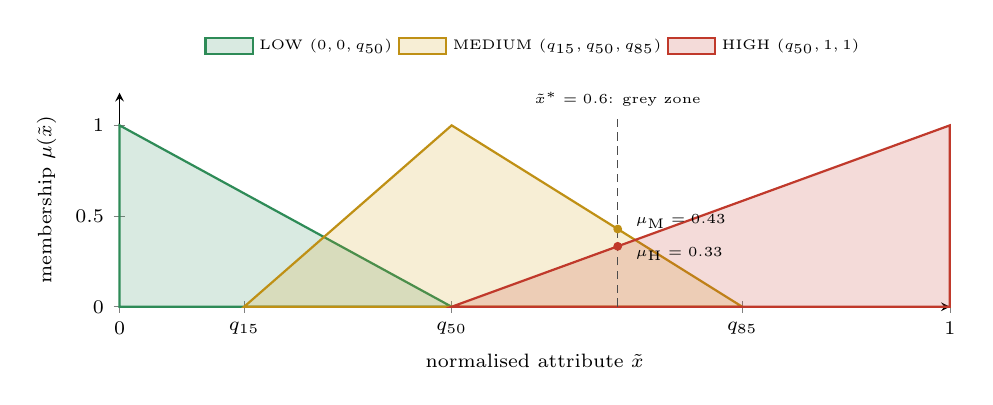
\begin{tikzpicture}
\begin{axis}[
  width=\columnwidth, height=4.3cm,
  xmin=0, xmax=1, ymin=0, ymax=1.18,
  xtick={0,0.15,0.4,0.75,1}, xticklabels={0,$q_{15}$,$q_{50}$,$q_{85}$,1},
  ytick={0,0.5,1}, tick label style={font=\scriptsize},
  xlabel={normalised attribute $\tilde{x}$}, ylabel={membership $\mu(\tilde{x})$},
  label style={font=\scriptsize},
  legend style={font=\tiny, draw=none, fill=none, at={(0.5,1.13)}, anchor=south, legend columns=3},
  area legend, axis lines=left, clip=false]
  \addplot[draw=nrm, thick, fill=nrm, fill opacity=0.18] coordinates {(0,1) (0.4,0)} \closedcycle;
  \addlegendentry{LOW $(0,0,q_{50})$}
  \addplot[draw=sus!90!black, thick, fill=sus, fill opacity=0.18] coordinates {(0.15,0) (0.4,1) (0.75,0)} \closedcycle;
  \addlegendentry{MEDIUM $(q_{15},q_{50},q_{85})$}
  \addplot[draw=atk, thick, fill=atk, fill opacity=0.18] coordinates {(0.4,0) (1,1)} \closedcycle;
  \addlegendentry{HIGH $(q_{50},1,1)$}
  \draw[densely dashed, black!70] (axis cs:0.6,0) -- (axis cs:0.6,1.05);
  \fill[sus!90!black] (axis cs:0.6,0.4286) circle (1.6pt);
  \fill[atk] (axis cs:0.6,0.3333) circle (1.6pt);
  \node[font=\tiny, anchor=west] at (axis cs:0.61,0.47) {$\mu_{\mathrm{M}}=0.43$};
  \node[font=\tiny, anchor=west] at (axis cs:0.61,0.29) {$\mu_{\mathrm{H}}=0.33$};
  \node[font=\tiny, anchor=south] at (axis cs:0.6,1.05) {$\tilde{x}^{\ast}=0.6$: grey zone};
\end{axis}
\end{tikzpicture}
\caption{Data-driven triangular membership functions placed at training percentiles (illustrative $q$ values). A borderline window ($\tilde{x}^{\ast}=0.6$) is simultaneously MEDIUM (0.43) and HIGH (0.33) instead of being forced to one side of a crisp threshold.}
\label{fig:mf}
\end{figure}

\subsection{Direction-Gated Expert Rule Base}
Eight Mamdani-style rules encode the flood signatures of Section~\ref{sec:related}. Each rule is the $\min$ t-norm of two (R8: three) antecedent grades, gated by the LOW grade of the response direction:
\begin{equation}
  R_k=\min\!\big(\mu_{A_k},\,\mu_{B_k},\,\mu^{\mathrm{LOW}}_{d}\big),\qquad k=1,\dots,8.
\end{equation}
The gate means that a victim's reply ($d_i=1$, so $\mu^{\mathrm{LOW}}_{d}=0$) can never fire an attack rule, which guarantees attacker-direction attribution (goal G4). Table~\ref{tab:rules} lists the rules together with how often each one fires on the held-out data. The rule evidence is summarised in a fuzzy confidence that blends weighted evidence with the strongest single rule:
\begin{equation}
  c=0.55\sum_{k=1}^{8}w_kR_k+0.45\max_k R_k,\qquad \textstyle\sum_k w_k=1.
  \label{eq:fconf}
\end{equation}

\begin{table}[t]
\centering
\caption{Direction-gated rule base: weights and held-out firing rates ($R_k>0.1$) on attack vs.\ normal packets}
\label{tab:rules}
\footnotesize
\renewcommand{\arraystretch}{1.1}
\setlength{\tabcolsep}{3.2pt}
\begin{tabular}{@{}l >{\raggedright\arraybackslash}p{3.75cm} c r r@{}}
\toprule
\textbf{Rule} & \textbf{Antecedent} ($\wedge\,d$ is LOW) & $w_k$ & \textbf{Atk.} & \textbf{Norm.} \\
\midrule
R1 & SYN/ACK HIGH $\wedge$ half-open HIGH & 0.16 & 63.9\% & 15.2\% \\
R2 & SYN density HIGH $\wedge$ inter-SYN LOW & 0.15 & 62.3\% & 11.8\% \\
R3 & src frequency LOW $\wedge$ SYN/ACK HIGH & 0.12 & 0.0\% & 0.0\% \\
R4 & SYN density HIGH $\wedge$ half-open HIGH & 0.10 & 56.8\% & 10.9\% \\
R5 & dst-port diversity LOW $\wedge$ SYN density HIGH & 0.10 & 11.8\% & 0.3\% \\
R6 & UDP density HIGH $\wedge$ pkt density HIGH & 0.15 & 0.0\% & 7.7\% \\
R7 & byte density HIGH $\wedge$ pkt density HIGH & 0.12 & 21.4\% & 3.0\% \\
R8 & UDP, SYN/ACK, pkt density all MEDIUM & 0.10 & 8.6\% & 2.4\% \\
\midrule
$c$ & fuzzy confidence, Eq.~\eqref{eq:fconf} & -- & 72.5\% & 25.3\% \\
\bottomrule
\end{tabular}
\end{table}

\subsection{Lightweight Fuzzy Decision Tree}
The tree sees \emph{only} the fuzzy space,
\begin{equation}
  \mathbf{z}_i=\big[\,\boldsymbol{\mu}_i\;(30),\;\mathbf{R}_i\;(8),\;c_i\;(1)\,\big]\in[0,1]^{39}.
\end{equation}
Every split therefore reads as a linguistic condition, e.g., ``$\mu^{\mathrm{HIGH}}(\text{byte density})>0.18$''. Every root-to-leaf path becomes an IF-THEN rule, as in Fuzzy-ID3~\cite{ye2022,yuan1995}. Classical Fuzzy-ID3 propagates membership degrees through a fuzzy-entropy criterion. We instead run crisp CART induction~\cite{breiman1984} over the fuzzified features. This keeps inference to at most nine comparisons and lets the baseline tree be trained by \emph{exactly} the same procedure (Algorithm~\ref{alg:fdt}). A grid of 60 configurations is scored by 3-fold stratified cross-validated F1 on the training set. Cost-complexity pruning, which minimises $R_\alpha(T)=R(T)+\alpha|\tilde{T}|$, then selects the \emph{smallest} tree whose CV-F1 lies within $\delta=0.005$ of the best:
\begin{equation}
  \alpha^{\star}=\arg\min_{\alpha}\;|T_\alpha|\quad\text{s.t.}\quad \mathrm{F1}_{\mathrm{CV}}(T_\alpha)\ge\mathrm{F1}^{\star}_{\mathrm{CV}}-\delta.
\end{equation}
The selected configuration (depth 10, minimum leaf 5, class weight 1:4) is pruned with $\alpha^{\star}=1.67\times10^{-4}$ from 371 to \textbf{89 nodes}. The result has depth 9 and 45 leaves and uses 20 of the 39 fuzzy features.

\begin{algorithm}[t]
\caption{Shared lightweight tree training and rule fusion}
\label{alg:fdt}
\begin{algorithmic}[1]
\Require training features $Z$ (fuzzy) or $X$ (raw); labels $y$; fuzzy confidence $c$
\Ensure pruned tree $T$; fusion weight $\lambda$; threshold $\tau$
\State $\mathcal{G}\gets\{4,6,8,10,12\}\times\{5,20,40\}\times\{1{:}2,1{:}3,1{:}4,\text{bal.}\}$
\State $g^\star\gets\arg\max_{g\in\mathcal{G}}\mathrm{F1}_{\mathrm{CV}}(g)$ \Comment{3-fold stratified}
\State $T_0\gets\textsc{Fit}(g^\star)$; compute CCP path $\{\alpha_j\}$
\State $T\gets$ smallest $T_{\alpha_j}$ with $\mathrm{F1}_{\mathrm{CV}}\ge\mathrm{F1}_{\mathrm{CV}}(g^\star)-0.005$
\For{$\lambda\in\{0,0.3,0.5,0.6,0.7,0.8,1\}$}
  \State $s\gets\max(p_T(Z),\lambda c)$
  \State $(\tau_\lambda,J_\lambda)\gets\arg\max_{\tau}J(\tau;s,y)$ s.t.\ recall $\ge0.35$
\EndFor
\State \Return $T,\;\lambda^\star=\arg\max_\lambda J_\lambda,\;\tau_{\lambda^\star}$
\end{algorithmic}
\end{algorithm}

\subsection{Rule Fusion and Decision}
The deployed threat score fuses the tree's posterior with the rule evidence,
\begin{equation}
  s=\max\!\big(p_T(\mathbf{z}),\;\lambda\,c\big),
  \label{eq:fusion}
\end{equation}
so that windows where the tree is uncertain but expert rules fire strongly can still be escalated. The pair $(\lambda,\tau)$ maximises a single operating-point objective on the \emph{training} predictions:
\begin{equation}
  J(\tau)=0.5\,\mathrm{F1}+0.3\,\mathrm{Acc}+0.2\,\mathrm{BAcc},\quad \text{recall}\ge0.35,
  \label{eq:objective}
\end{equation}
which gives $\lambda=0.7$ and $\tau=0.48$. Every baseline model is thresholded with the same objective.

\subsection{Forensic Rule Extraction}
Following Ye~\cite{ye2022}, every root-to-leaf path is exported as an IF-THEN rule whose confidence is the leaf purity. The deployed tree yields 45 rules. The 16 attack rules have a mean length of 6.8 conditions (6 to 9). Fig.~\ref{fig:fuzzypipe} summarises the reasoning chain, and Section~\ref{sec:case} traces a real held-out verdict.

% ---------------------------------------------------------------------
% FIGURE 6 : fuzzy reasoning pipeline
% ---------------------------------------------------------------------
\begin{figure*}[t]
\centering
\resizebox{\textwidth}{!}{%
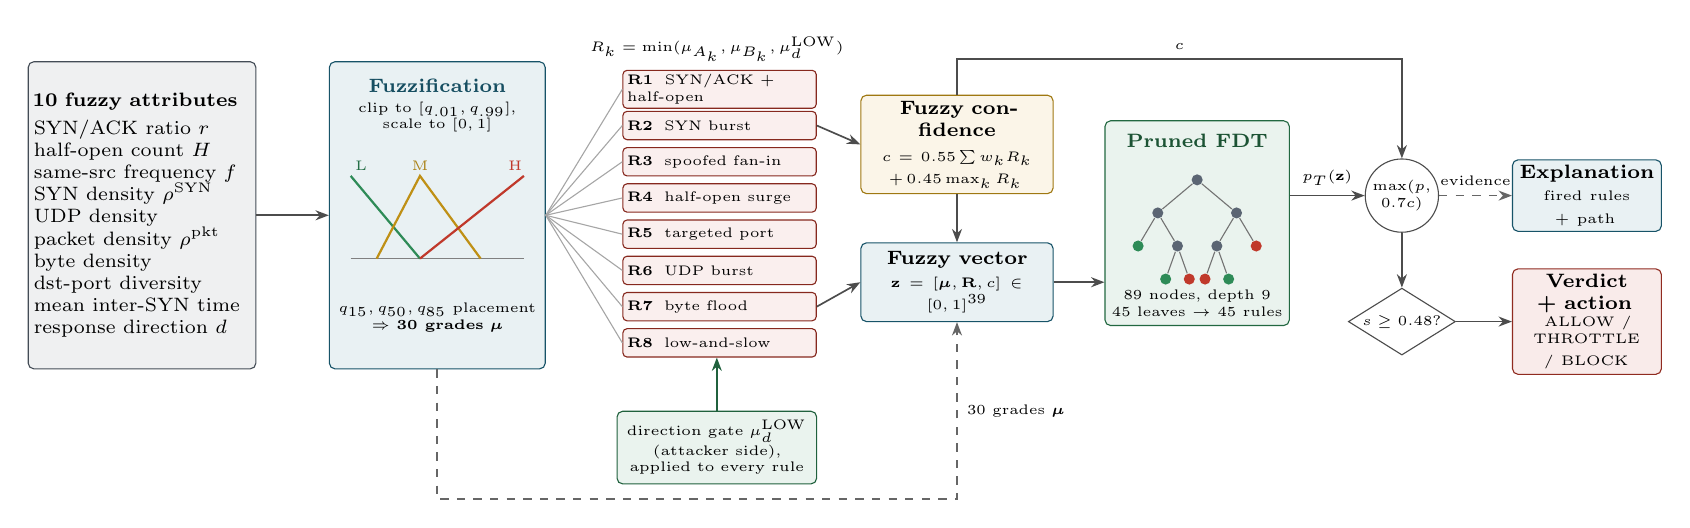
\begin{tikzpicture}[font=\scriptsize]
  % column A: attributes
  \node[box=gr, text width=2.75cm, minimum height=3.9cm, align=left] (A) at (0,0) {%
    \textbf{10 fuzzy attributes}\\[2pt]
    SYN/ACK ratio $r$\\ half-open count $H$\\ same-src frequency $f$\\ SYN density $\rho^{\mathrm{SYN}}$\\ UDP density\\ packet density $\rho^{\mathrm{pkt}}$\\ byte density\\ dst-port diversity\\ mean inter-SYN time\\ response direction $d$};
  % column B: membership bank
  \node[box=fz, text width=2.6cm, minimum height=3.9cm] (B) at (3.75,0) {};
  \node[font=\scriptsize\bfseries, text=fz!70!black] at (3.75,1.65) {Fuzzification};
  \node[font=\tiny, align=center] at (3.75,1.25) {clip to $[q_{.01},q_{.99}]$,\\scale to $[0,1]$};
  \begin{scope}[shift={(2.65,-0.55)}, x=2.2cm, y=1.05cm]
    \draw[black!50] (0,0) -- (1,0);
    \draw[nrm, thick] (0,1) -- (0.4,0);
    \draw[sus!90!black, thick] (0.15,0) -- (0.4,1) -- (0.75,0);
    \draw[atk, thick] (0.4,0) -- (1,1);
    \node[font=\tiny, text=nrm!80!black] at (0.06,1.12) {L};
    \node[font=\tiny, text=sus!80!black] at (0.4,1.12) {M};
    \node[font=\tiny, text=atk] at (0.95,1.12) {H};
  \end{scope}
  \node[font=\tiny, align=center] at (3.75,-1.3) {$q_{15},q_{50},q_{85}$ placement\\$\Rightarrow$ \textbf{30 grades} $\boldsymbol{\mu}$};
  % column C: rules
  \foreach \k/\t [count=\j from 0] in {R1/{SYN/ACK + half-open},R2/SYN burst,R3/spoofed fan-in,R4/half-open surge,R5/targeted port,R6/UDP burst,R7/byte flood,R8/low-and-slow}{
    \node[draw=atk!70!black, fill=atk!8, rounded corners=1.5pt, font=\tiny, text width=2.35cm,
          minimum height=0.36cm, inner sep=1.5pt, anchor=west] (R\j) at (6.1,1.6-\j*0.46) {\textbf{\k}\; \t};
  }
  \node[draw=nrm!70!black, fill=nrm!10, rounded corners=2pt, font=\tiny, align=center, text width=2.3cm] (G) at (7.3,-2.95)
     {direction gate $\mu^{\mathrm{LOW}}_{d}$ (attacker side), applied to every rule};
  \draw[arr, draw=nrm!70!black] (G.north) -- (G.north |- R7.south);
  \node[font=\tiny, anchor=south] at (7.3,1.83) {$R_k=\min(\mu_{A_k},\mu_{B_k},\mu^{\mathrm{LOW}}_d)$};
  % column D: aggregation
  \node[box=sus, text width=2.3cm, minimum height=1.2cm] (C) at (10.35,0.9) {\textbf{Fuzzy confidence}\\[1pt]{\tiny $c=0.55\sum w_kR_k$}\\{\tiny $+\,0.45\max_kR_k$}};
  \node[box=fz, text width=2.3cm, minimum height=1.0cm] (Z) at (10.35,-0.85) {\textbf{Fuzzy vector}\\{\tiny $\mathbf{z}=[\boldsymbol{\mu},\mathbf{R},c]\in[0,1]^{39}$}};
  % column E: tree
  \node[box=nrm, text width=2.2cm, minimum height=2.6cm] (T) at (13.4,-0.1) {};
  \node[font=\scriptsize\bfseries, text=nrm!60!black] at (13.4,0.95) {Pruned FDT};
  \begin{scope}[shift={(13.4,0.45)}, every node/.style={circle, inner sep=0pt, minimum size=4pt}]
    \node[fill=gr] (n0) at (0,0) {};
    \node[fill=gr] (n1) at (-0.5,-0.42) {}; \node[fill=gr] (n2) at (0.5,-0.42) {};
    \node[fill=nrm] (n3) at (-0.75,-0.84) {}; \node[fill=gr] (n4) at (-0.25,-0.84) {};
    \node[fill=gr] (n5) at (0.25,-0.84) {}; \node[fill=atk] (n6) at (0.75,-0.84) {};
    \node[fill=nrm] (n7) at (-0.4,-1.26) {}; \node[fill=atk] (n8) at (-0.1,-1.26) {};
    \node[fill=atk] (n9) at (0.1,-1.26) {}; \node[fill=nrm] (n10) at (0.4,-1.26) {};
    \foreach \a/\b in {n0/n1,n0/n2,n1/n3,n1/n4,n2/n5,n2/n6,n4/n7,n4/n8,n5/n9,n5/n10} \draw[black!55] (\a) -- (\b);
  \end{scope}
  \node[font=\tiny, align=center] at (13.4,-1.12) {89 nodes, depth 9\\45 leaves $\to$ 45 rules};
  % column F: fusion + decision
  \node[draw=black!70, fill=white, circle, font=\tiny, inner sep=1pt, align=center] (M) at (16.0,0.25) {$\max(p,$\\$0.7c)$};
  \node[draw=black!70, fill=white, diamond, aspect=1.6, font=\tiny, inner sep=0.5pt] (D) at (16.0,-1.35) {$s\ge0.48$?};
  \node[box=fz, text width=1.75cm, minimum height=0.85cm] (E) at (18.35,0.25) {\textbf{Explanation}\\{\tiny fired rules + path}};
  \node[box=atk, text width=1.75cm, minimum height=0.85cm] (V) at (18.35,-1.35) {\textbf{Verdict + action}\\{\tiny ALLOW / THROTTLE\\/ BLOCK}};
  % arrows
  \draw[arr] (A.east) -- (B.west);
  \foreach \j in {0,...,7} \draw[black!35] (B.east) -- (R\j.west);
  \draw[arr] (R1.east) -- (C.west);
  \draw[arr] (R6.east) -- (Z.west);
  \draw[arr] (C.south) -- (Z.north);
  \draw[darr] (B.south) -- ++(0,-1.65) -| node[pos=0.75, right, font=\tiny] {30 grades $\boldsymbol{\mu}$} (Z.south);
  \draw[arr] (Z.east) -- (T.west |- Z.east);
  \draw[arr] (T.east |- M) -- node[above, font=\tiny] {$p_T(\mathbf{z})$} (M.west);
  \draw[arr] (C.north) -- ++(0,0.45) -| node[pos=0.25, above, font=\tiny] {$c$} (M.north);
  \draw[arr] (M.south) -- (D.north);
  \draw[darr] (M.east) -- node[above, font=\tiny] {evidence} (E.west);
  \draw[arr] (D.east) -- (V.west);
\end{tikzpicture}}
\caption{Fuzzy reasoning pipeline of \fname{}. Normalised attributes are fuzzified into 30 grades. Eight direction-gated rules ($\min$ t-norm) produce named attack evidence that is summarised by the fuzzy confidence $c$. A pruned tree trained only on the 39-dimensional fuzzy vector gives $p_T$, and the fused score $\max(p_T,0.7c)$ selects the response. The fired rules and the decision path form the explanation.}
\label{fig:fuzzypipe}
\end{figure*}

% =====================================================================
\section{Edge Deployment and Graduated Response}
\label{sec:edge}

\subsection{Live Detection Engine}
The research pipeline runs on a laptop. The Raspberry Pi only loads the artifact, which contains the pruned tree, the feature order, the clip bounds, the membership parameters, $\lambda$, $\tau$ and $W$. The engine (\texttt{live\_detector.py}) runs a scapy~\cite{scapy} sniffer thread with a BPF filter (e.g., \texttt{ip and not port 22}) that feeds a bounded queue, so a flood cannot exhaust memory. A worker thread maintains the 50-packet window. It recomputes the 22 features in pure Python ($\approx$1\,ms per window, without pandas) using \emph{the same arithmetic as training}, which avoids train/serve skew. It then applies the frozen fuzzy layer and scores the window with Eq.~\eqref{eq:fusion}. No verdicts are issued until 20 packets have been seen (warm-up). A deterministic replay mode (\texttt{-{}-replay-csv}) supports reproducible tests.

\subsection{Graduated, Reversible Response}
Each score is attributed to the dominant source of the window, and a per-source state machine (Fig.~\ref{fig:fsm}) is updated:
\begin{equation}
  a(s)=\begin{cases}
   \textsc{Block}, & s\ge\tau\\
   \textsc{Throttle}, & \tau/2\le s<\tau\\
   \textsc{Allow}, & s<\tau/2 .
  \end{cases}
\end{equation}
THROTTLE issues a rate-limit advisory with a 20\,s TTL, for low-level floods that warrant active monitoring. BLOCK installs an \texttt{iptables} DROP rule (with \texttt{-{}-live-firewall}; otherwise the block is simulated and logged) with a 120\,s TTL and automatic release. This graduated design follows the analyst-triage practice of escalating HIGH threats while only monitoring MEDIUM ones. It keeps a single false alarm from becoming a permanent outage.

% ---------------------------------------------------------------------
% FIGURE 7 : response state machine
% ---------------------------------------------------------------------
\begin{figure}[t]
\centering
\resizebox{\columnwidth}{!}{%
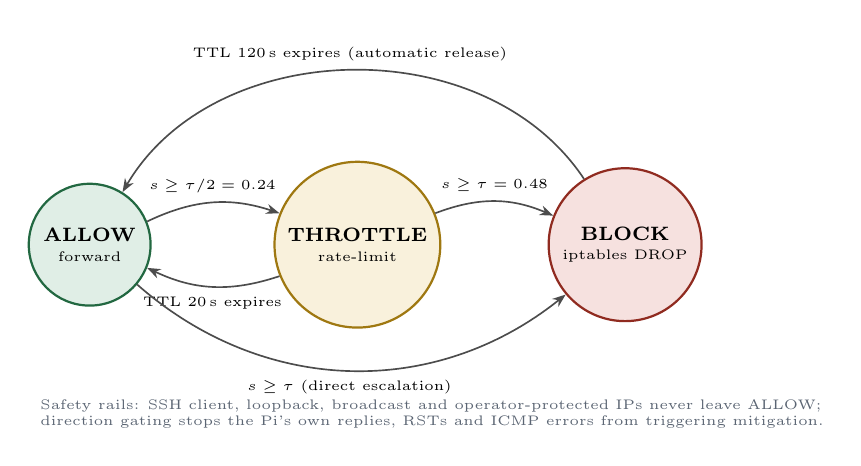
\begin{tikzpicture}[font=\scriptsize]
  \node[fsmstate=nrm] (al) at (0,0) {ALLOW\\[-1pt]{\tiny\mdseries forward}};
  \node[fsmstate=sus] (th) at (3.4,0) {THROTTLE\\[-1pt]{\tiny\mdseries rate-limit}};
  \node[fsmstate=atk] (bl) at (6.8,0) {BLOCK\\[-1pt]{\tiny\mdseries iptables DROP}};
  \draw[arr] (al) to[bend left=22] node[above, font=\tiny] {$s\ge\tau/2=0.24$} (th);
  \draw[arr] (th) to[bend left=22] node[above, font=\tiny] {$s\ge\tau=0.48$} (bl);
  \draw[arr] (th) to[bend left=22] node[below, font=\tiny] {TTL 20\,s expires} (al);
  \draw[arr] (al) to[bend right=40] node[below, font=\tiny] {$s\ge\tau$ (direct escalation)} (bl);
  \draw[arr] (bl) to[bend right=58] node[above, font=\tiny] {TTL 120\,s expires (automatic release)} (al);
  \node[font=\tiny, text=gr, align=left, anchor=west] at (-0.75,-2.15) {Safety rails: SSH client, loopback, broadcast and operator-protected IPs never leave ALLOW;\\direction gating stops the Pi's own replies, RSTs and ICMP errors from triggering mitigation.};
\end{tikzpicture}}
\caption{Per-source graduated response. Escalation follows the fused threat score, and every mitigation expires automatically after its TTL.}
\label{fig:fsm}
\end{figure}

\subsection{Safety Rails and Forensic Logging}
The SSH client address (taken from \texttt{SSH\_CLIENT}), loopback, broadcast and operator-supplied \texttt{-{}-protect} addresses are never blocked. Direction gating ensures that the Pi's own SYN-ACKs, RSTs and ICMP errors cannot trigger mitigation. Each decision is appended to a JSON-lines event log with the timestamp, score, tree probability, fuzzy confidence, all eight rule activations, the window statistics, the dominant source and the action taken. Packet events are rate-limited so that a flood cannot inflate the log. An atomic state snapshot is written every second. Together these provide a time-ordered evidence trail for the preservation and presentation stages of the forensic process model~\cite{naing2023,ye2022}.

\subsection{Dashboard and Traffic Simulator}
A dependency-free dashboard (Python standard-library HTTP) runs on the Pi. It shows KPI cards, the live packet stream, a per-IP threat board with manual block/release controls, score timelines, the fired-rule explanation of each decision, CPU/RAM/temperature telemetry and the benchmark table. A companion simulator generates \emph{normal}, \emph{suspicious} (low-and-slow scan), \emph{low-flood}, \emph{congestion}, \emph{syn-flood} and \emph{udp-flood} traffic, plus a scripted \emph{story} mode that logs ground-truth timestamps for time-to-detect scoring. The congestion scenario uses complete TCP handshakes at a high rate and therefore serves as a built-in false-positive test.

% =====================================================================
\section{Experimental Setup}
\label{sec:setup}

\textbf{Models.} All models are evaluated on the same chronological hold-out (38,747 packets, 2,962 attacks) and thresholded with the same objective, Eq.~\eqref{eq:objective}, tuned on the training data only.
\begin{itemize}
  \item \textbf{Fuzzy DT (proposed, deployed):} 39 fuzzy features, Algorithm~\ref{alg:fdt}, fused score with $\lambda=0.7$.
  \item \textbf{Plain DT:} the 22 raw features, trained by the \emph{identical} Algorithm~\ref{alg:fdt}. It selects the same configuration and is pruned from 463 to 71 nodes. The only difference from the proposed model is the feature space.
  \item \textbf{Deep MLP:} hidden layers 256-128-64-32 with ReLU, Adam (learning rate $5\times10^{-4}$, adaptive), L2 penalty $10^{-4}$, batch size 256, early stopping (15\% validation data, patience 25), standardised inputs and attack oversampling to 1:2.
  \item \textbf{Fuzzy Forest (reference):} 30 trees~\cite{breiman2001} (depth 14, balanced subsampling) on the same 39 fuzzy features, fused with $\lambda=1$.
\end{itemize}
\textbf{Metrics.} We report accuracy, balanced accuracy (BAcc), precision, recall and F1 for the attack class, ROC-AUC computed on each model's probability output, false-positive rate (FPR), serialised model size, and per-packet latency. Latency is the median of 5 vectorised runs over 2,000 held-out packets on the real artifacts, including the fuzzification step.
\textbf{Software.} Python~3.12, scikit-learn~\cite{pedregosa2011}, NumPy, pandas, joblib and scapy~\cite{scapy}. Training is done on a laptop, and inference runs on the Raspberry Pi under Raspberry Pi OS.

% =====================================================================
\section{Results and Discussion}
\label{sec:results}

\subsection{Overall Comparison}
Table~\ref{tab:main} and Fig.~\ref{fig:bars} summarise the hold-out results. The deployed Fuzzy DT achieves the best accuracy among the single models (87.74\%), the best precision (34.51\%) and the best F1 of all four models (0.456). It improves on the identically trained plain DT by $+1.35$ accuracy points, $+2.54$ precision points and $+0.019$ F1. It also beats the deep MLP on accuracy, precision and F1 while being $125\times$ smaller (9.1\,KB vs.\ 1.14\,MB). The Fuzzy Forest gains $+0.55$ accuracy points over the single tree but loses 0.014 F1 and 6.6 recall points, at roughly $300\times$ the size (35,478 vs.\ 89 nodes). The single pruned tree is therefore the right choice for the edge.

The plain DT has the highest ROC-AUC (0.917). The Fuzzy DT's tree probability scores 0.908, and its deployed fused score scores 0.911. All models are thus close in ranking quality. The fuzzy representation pays off at the \emph{operating point}: at the tuned threshold it converts the same ranking ability into fewer false alarms.

\begin{table*}[t]
\centering
\caption{Hold-out results (38,747 packets, 7.64\% attack). Best value per column in bold. Latency is per packet and includes fuzzification}
\label{tab:main}
\footnotesize
\renewcommand{\arraystretch}{1.12}
\begin{tabular}{@{}l l r r r r r r r r r@{}}
\toprule
\textbf{Model} & \hd{\textbf{Feature}\\\textbf{space}} & \hd{\textbf{Acc.}\\\textbf{(\%)}} & \hd{\textbf{BAcc}\\\textbf{(\%)}} & \hd{\textbf{Prec.}\\\textbf{(\%)}} & \hd{\textbf{Recall}\\\textbf{(\%)}} & \textbf{F1} & \textbf{AUC} & \hd{\textbf{FPR}\\\textbf{(\%)}} & \textbf{Size} & \hd{\textbf{Latency}\\\textbf{per pkt}} \\
\midrule
\textbf{Fuzzy DT (proposed, deployed)} & 39 fuzzy & 87.74 & 78.34 & 34.51 & 67.25 & \textbf{0.456} & 0.908 & 10.57 & 9.1\,KB & 13.4\,$\mu$s \\
Fuzzy Forest, 30 trees (reference) & 39 fuzzy & \textbf{88.29} & 75.64 & \textbf{34.78} & 60.70 & 0.442 & 0.912 & \textbf{9.42} & 2.72\,MB & 24.0\,$\mu$s \\
Plain DT (identical protocol) & 22 raw & 86.39 & 78.52 & 31.97 & 69.24 & 0.438 & \textbf{0.917} & 12.20 & 7.1\,KB & \textbf{0.76\,$\mu$s} \\
Deep MLP (256-128-64-32) & 22 raw & 86.51 & \textbf{78.67} & 32.24 & \textbf{69.41} & 0.440 & 0.911 & 12.08 & 1.14\,MB & 5.05\,$\mu$s \\
\bottomrule
\end{tabular}
\end{table*}

% ---------------------------------------------------------------------
% FIGURE 8 : result bar charts
% ---------------------------------------------------------------------
\begin{figure*}[t]
\centering
\resizebox{\textwidth}{!}{%
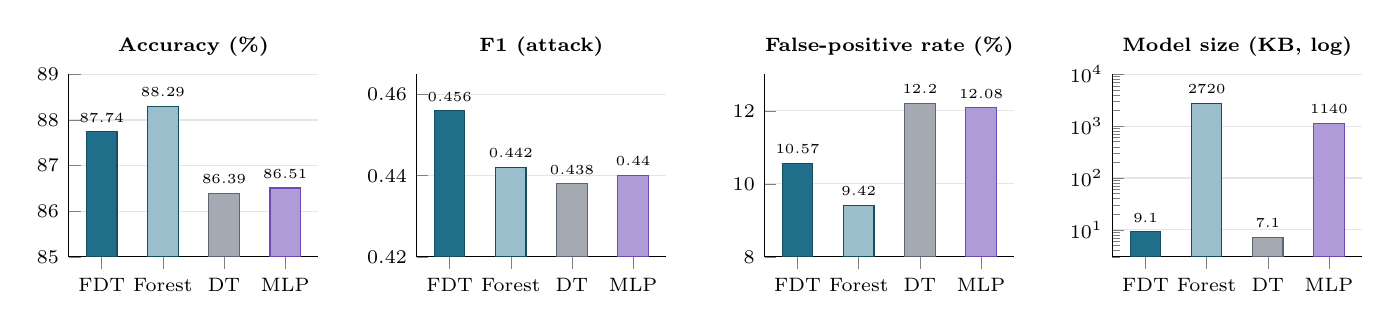
\begin{tikzpicture}
\begin{groupplot}[
  group style={group size=4 by 1, horizontal sep=1.25cm},
  width=4.75cm, height=3.9cm, every axis/.append style={ybar, bar width=11pt}, every axis plot post/.append style={bar shift=0pt},
  symbolic x coords={FDT,Forest,DT,MLP}, xtick={FDT,Forest,DT,MLP},
  tick label style={font=\scriptsize}, label style={font=\scriptsize},
  title style={font=\scriptsize\bfseries, yshift=-3pt},
  nodes near coords, nodes near coords style={font=\tiny, /pgf/number format/fixed},
  enlarge x limits=0.18, axis x line*=bottom, axis y line*=left,
  ymajorgrids, grid style={black!10}]
\nextgroupplot[title={Accuracy (\%)}, ymin=85, ymax=89,
   nodes near coords style={font=\tiny, /pgf/number format/.cd, fixed, precision=2}]
  \addplot[fill=fz, draw=fz!70!black] coordinates {(FDT,87.74)};
  \addplot[fill=fz!45, draw=fz!70!black] coordinates {(Forest,88.29)};
  \addplot[fill=gr!55, draw=gr] coordinates {(DT,86.39)};
  \addplot[fill=vio!55, draw=vio] coordinates {(MLP,86.51)};
\nextgroupplot[title={F1 (attack)}, ymin=0.42, ymax=0.465,
   nodes near coords style={font=\tiny, /pgf/number format/.cd, fixed, precision=3}]
  \addplot[fill=fz, draw=fz!70!black] coordinates {(FDT,0.456)};
  \addplot[fill=fz!45, draw=fz!70!black] coordinates {(Forest,0.442)};
  \addplot[fill=gr!55, draw=gr] coordinates {(DT,0.438)};
  \addplot[fill=vio!55, draw=vio] coordinates {(MLP,0.440)};
\nextgroupplot[title={False-positive rate (\%)}, ymin=8, ymax=13,
   nodes near coords style={font=\tiny, /pgf/number format/.cd, fixed, precision=2}]
  \addplot[fill=fz, draw=fz!70!black] coordinates {(FDT,10.57)};
  \addplot[fill=fz!45, draw=fz!70!black] coordinates {(Forest,9.42)};
  \addplot[fill=gr!55, draw=gr] coordinates {(DT,12.20)};
  \addplot[fill=vio!55, draw=vio] coordinates {(MLP,12.08)};
\nextgroupplot[title={Model size (KB, log)}, ymode=log, ymin=3, ymax=10000, log origin=infty,
   nodes near coords style={font=\tiny, /pgf/number format/.cd, fixed, precision=1},
   point meta=explicit symbolic]
  \addplot[fill=fz, draw=fz!70!black] coordinates {(FDT,9.1) [9.1]};
  \addplot[fill=fz!45, draw=fz!70!black] coordinates {(Forest,2720) [2720]};
  \addplot[fill=gr!55, draw=gr] coordinates {(DT,7.1) [7.1]};
  \addplot[fill=vio!55, draw=vio] coordinates {(MLP,1140) [1140]};
\end{groupplot}
\end{tikzpicture}}
\caption{Hold-out comparison. The 9.1\,KB Fuzzy DT has the best F1, cuts false positives relative to both raw-feature baselines, and is $125\times$ smaller than the deep MLP and $300\times$ smaller than the Fuzzy Forest.}
\label{fig:bars}
\end{figure*}

\subsection{False Alarms and Per-Segment Behaviour}
Table~\ref{tab:confusion} lists the confusion counts. The Fuzzy DT raises 3,781 false alarms against 4,364 for the plain DT (583 fewer, $-13.4\%$) and 4,322 for the MLP (541 fewer). Fewer false alarms means less alert fatigue for the analyst and fewer wrongful blocks. All 3,781 false positives fall in the background segments, and \emph{none} fall on the victim's replies inside the attack phases. This is direct evidence that direction gating works. Recall is 98.4\% in the second flood segment but 55.5\% in the SYN-flood segment, which is the main target for improvement. Operationally, a source is blocked as soon as one of its windows crosses $\tau$, so a flood does not need to be detected packet by packet.

\begin{table}[t]
\centering
\caption{Confusion counts on the hold-out (2,962 attack / 35,785 normal)}
\label{tab:confusion}
\footnotesize
\renewcommand{\arraystretch}{1.08}
\setlength{\tabcolsep}{4.5pt}
\begin{tabular}{@{}l r r r r r@{}}
\toprule
\textbf{Model} & \textbf{TP} & \textbf{FN} & \textbf{FP} & \textbf{TN} & \textbf{FPR} \\
\midrule
\textbf{Fuzzy DT} & 1,992 & 970 & \textbf{3,781} & 32,004 & 10.57\% \\
Fuzzy Forest & 1,798 & 1,164 & 3,372 & 32,413 & 9.42\% \\
Plain DT & 2,051 & 911 & 4,364 & 31,421 & 12.20\% \\
Deep MLP & 2,056 & 906 & 4,322 & 31,463 & 12.08\% \\
\bottomrule
\end{tabular}
\end{table}

\subsection{Size, Accuracy and Latency}
Fig.~\ref{fig:pareto} plots F1 against model size. The Fuzzy DT is the only model in the top-left (small and accurate) corner. Its per-packet cost of 13.4\,$\mu$s is dominated by fuzzification. This is slower than the vectorised plain DT (0.76\,$\mu$s) and MLP (5.05\,$\mu$s), but it still sustains about 75,000 packets/s on one core. That is almost two orders of magnitude below the 1\,ms inter-arrival time of the $\approx$1,000\,pps floods in our capture, so the edge budget (G1) is comfortably met. Training-time pruning helped accuracy as well as size: the unpruned 371-node fuzzy tree scored 87.16\%, while the 89-node tree scores 87.74\%. On rolling-window data, regularisation rather than capacity drives generalisation.

% ---------------------------------------------------------------------
% FIGURE 9 : size vs F1 scatter
% ---------------------------------------------------------------------
\begin{figure}[t]
\centering
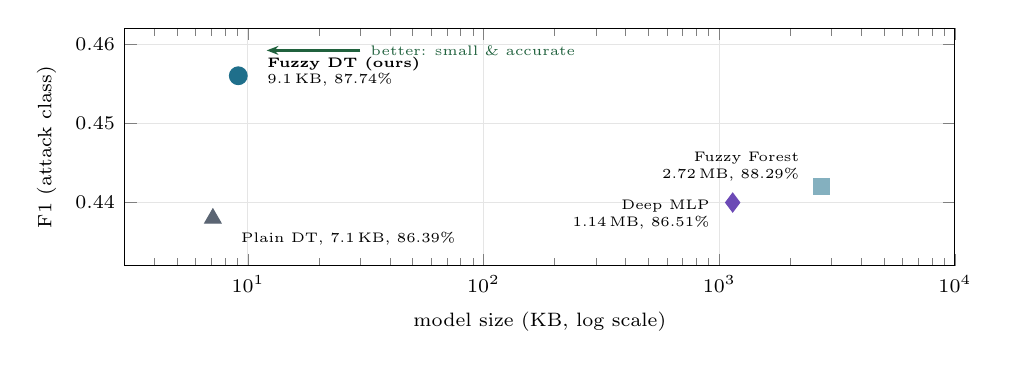
\begin{tikzpicture}
\begin{axis}[
  width=\columnwidth, height=4.6cm, xmode=log,
  xmin=3, xmax=10000, ymin=0.432, ymax=0.462,
  xlabel={model size (KB, log scale)}, ylabel={F1 (attack class)},
  tick label style={font=\scriptsize}, label style={font=\scriptsize},
  yticklabel style={/pgf/number format/.cd, fixed, precision=3},
  grid=major, grid style={black!10}, clip=false]
  \addplot[only marks, mark=*, mark size=3.2pt, color=fz] coordinates {(9.1,0.456)};
  \addplot[only marks, mark=square*, mark size=2.8pt, color=fz!55] coordinates {(2720,0.442)};
  \addplot[only marks, mark=triangle*, mark size=3.4pt, color=gr] coordinates {(7.1,0.438)};
  \addplot[only marks, mark=diamond*, mark size=3.4pt, color=vio] coordinates {(1140,0.440)};
  \node[font=\tiny, anchor=west, align=left] at (axis cs:11,0.4565) {\textbf{Fuzzy DT (ours)}\\9.1\,KB, 87.74\%};
  \node[font=\tiny, anchor=east, align=right] at (axis cs:2400,0.4445) {Fuzzy Forest\\2.72\,MB, 88.29\%};
  \node[font=\tiny, anchor=west, align=left] at (axis cs:8.5,0.4355) {Plain DT, 7.1\,KB, 86.39\%};
  \node[font=\tiny, anchor=east, align=right] at (axis cs:1000,0.4385) {Deep MLP\\1.14\,MB, 86.51\%};
  \draw[-{Stealth[length=1.5mm]}, nrm!70!black, thick] (axis cs:30,0.4592) -- (axis cs:12,0.4592)
     node[pos=0, right, font=\tiny, text=nrm!70!black] {better: small \& accurate};
\end{axis}
\end{tikzpicture}
\caption{F1 versus model size. The proposed tree dominates both raw-feature baselines and matches or beats models two to three orders of magnitude larger.}
\label{fig:pareto}
\end{figure}

\subsection{Ablation Study}
\label{sec:ablation}
Table~\ref{tab:ablation} isolates the components. (i) The \emph{expert rules alone}, thresholding $c$ with its own tuned threshold, behave like a hand-written fuzzy IDS. They reach a recall of 72.5\% but an FPR of 25.3\% and an F1 of only 0.303, which confirms that fixed rules are too blunt. (ii) Learning a pruned tree on top of the fuzzy space \emph{halves} the false-positive rate and lifts F1 by 0.149. (iii) Fusing the rules back in (Eq.~\eqref{eq:fusion}) recovers 22 more attacks with \emph{zero} additional false alarms. These are windows where the tree is uncertain but expert evidence is strong. (iv) With learner, grid, pruning and threshold held fixed, replacing the raw features with fuzzy ones accounts for the full gain over the plain DT. The improvement therefore comes from the representation, not from tuning. (v) Evaluation hygiene matters: a random split inflates the plain DT by 2.06 points, and training on the uncorrected weak labels depresses ROC-AUC to about 0.79. (vi) Data-driven membership placement matches hand-placed sets (train CV-F1 0.383 vs.\ 0.380) while removing every hand-tuned constant.

\begin{table}[t]
\centering
\caption{Ablations on the hold-out set (Acc.\ in \%)}
\label{tab:ablation}
\footnotesize
\renewcommand{\arraystretch}{1.08}
\setlength{\tabcolsep}{3.5pt}
\begin{tabular}{@{}l r r r r@{}}
\toprule
\textbf{Variant} & \textbf{Acc.} & \textbf{F1} & \textbf{Recall} & \textbf{FPR} \\
\midrule
Rules only ($c\ge0.09$) & 74.50 & 0.303 & 72.52 & 25.33 \\
Fuzzy tree only ($\lambda=0$) & 87.68 & 0.452 & 66.51 & 10.57 \\
\textbf{Fuzzy tree + rule fusion} ($\lambda=0.7$) & \textbf{87.74} & \textbf{0.456} & 67.25 & 10.57 \\
Unpruned fuzzy tree (371 nodes) & 87.16 & -- & -- & -- \\
Plain DT, raw features (honest split) & 86.39 & 0.438 & 69.24 & 12.20 \\
Plain DT, \emph{random} split (leaky) & 88.45 & -- & -- & -- \\
\bottomrule
\end{tabular}
\end{table}

\subsection{What the Tree Learned}
Fig.~\ref{fig:importance} shows the impurity-based feature importances of the deployed tree. The \emph{root} split is ``$c\le0.005$'', i.e., whether any direction-gated rule fired at all. The fuzzy confidence alone carries 35.4\% of the importance, and together with the direction grade more than half. The tree thus learned to \emph{trust and refine} the expert rules rather than replace them. The firing statistics in Table~\ref{tab:rules} show this as well. R1, R2 and R4 fire on 57--64\% of attack packets but only 11--15\% of normal packets. R5 (a single targeted port under a SYN burst) is the most specific rule (11.8\% vs.\ 0.3\%). R3 never fired because the captured attack came from one host, so source-dispersion evidence was absent. R6 fired only on background UDP/QUIC bursts, which explains part of the residual false alarms and motivates per-network recalibration.

% ---------------------------------------------------------------------
% FIGURE 10 : feature importances
% ---------------------------------------------------------------------
\begin{figure}[t]
\centering
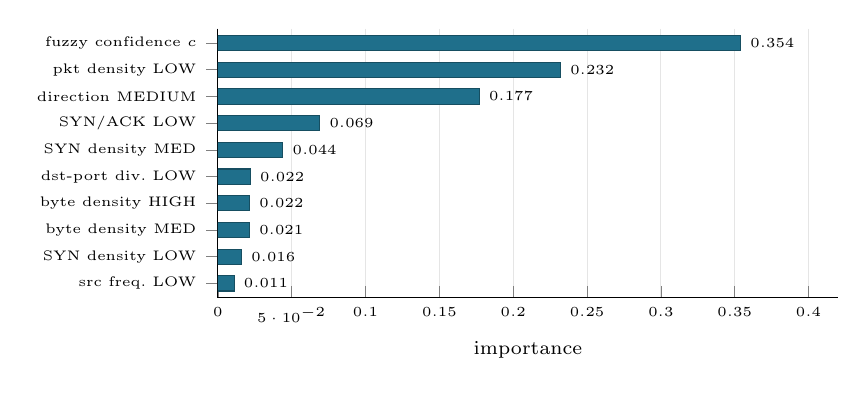
\begin{tikzpicture}
\begin{axis}[
  width=0.78\columnwidth, height=5.0cm, xbar, bar width=5.5pt,
  xmin=0, xmax=0.42, y dir=reverse,
  symbolic y coords={fconf,pktLOW,dirMED,saLOW,synMED,portLOW,byteHIGH,byteMED,synLOW,srcLOW},
  ytick=data,
  yticklabels={{fuzzy confidence $c$},{pkt density LOW},{direction MEDIUM},{SYN/ACK LOW},{SYN density MED},{dst-port div.\ LOW},{byte density HIGH},{byte density MED},{SYN density LOW},{src freq.\ LOW}},
  tick label style={font=\tiny}, xlabel={importance}, label style={font=\scriptsize},
  nodes near coords, nodes near coords style={font=\tiny, /pgf/number format/.cd, fixed, precision=3},
  axis x line*=bottom, axis y line*=left, xmajorgrids, grid style={black!10},
  enlarge y limits=0.06]
  \addplot[fill=fz, draw=fz!70!black] coordinates {
    (0.354,fconf) (0.232,pktLOW) (0.177,dirMED) (0.069,saLOW) (0.044,synMED)
    (0.022,portLOW) (0.0215,byteHIGH) (0.0214,byteMED) (0.016,synLOW) (0.011,srcLOW)};
\end{axis}
\end{tikzpicture}
\caption{Top-10 feature importances of the deployed Fuzzy DT. The rule-layer output (fuzzy confidence) is the root split and the most important feature.}
\label{fig:importance}
\end{figure}

\subsection{Case Study: Anatomy of a Forensic Verdict}
\label{sec:case}
Fig.~\ref{fig:case} traces a real held-out packet from the SYN-flood phase through the deployed tree. The raw window shows a SYN to port~80 with TCP window 512 and zero payload, 38 half-open connections out of 50 packets, saturated SYN and packet densities, and a 0.18\,ms mean inter-SYN gap. Rules R1 and R4 fire fully, R2 at 0.84, R5 at 0.50 and R7 at 0.31, giving $c=0.71$. The tree path (six conditions) ends in a pure attack leaf supported by 53 training windows. The fused score is $s=\max(1.0,0.7\times0.71)=1.0\ge\tau$, so the source is blocked. The exported rule reads like an analyst's note:

\smallskip
\noindent\fbox{\parbox{0.96\columnwidth}{\footnotesize\ttfamily
IF fuzzy evidence present (c=0.71)\\
\hspace*{1em}AND SYN/ACK ratio is NOT low ($\mu$=0.00)\\
\hspace*{1em}AND SYN density is NOT medium ($\mu$=0.00)\\
\hspace*{1em}AND byte density is HIGH ($\mu$=0.31)\\
\hspace*{1em}AND SYN-burst rule R2 holds ($\mu$=0.84)\\
\hspace*{1em}AND dst-port diversity is LOW ($\mu$=0.50)\\
THEN TCP-SYN flood [leaf purity 100\%, n=53]\\
ACTION: BLOCK src, iptables DROP, TTL 120 s}}
\smallskip

\noindent An equally accurate MLP would offer only a probability. Here every term maps to an indicator a forensic examiner already uses~\cite{naing2023}.

% ---------------------------------------------------------------------
% FIGURE 11 : case study
% ---------------------------------------------------------------------
\begin{figure*}[t]
\centering
\resizebox{\textwidth}{!}{%
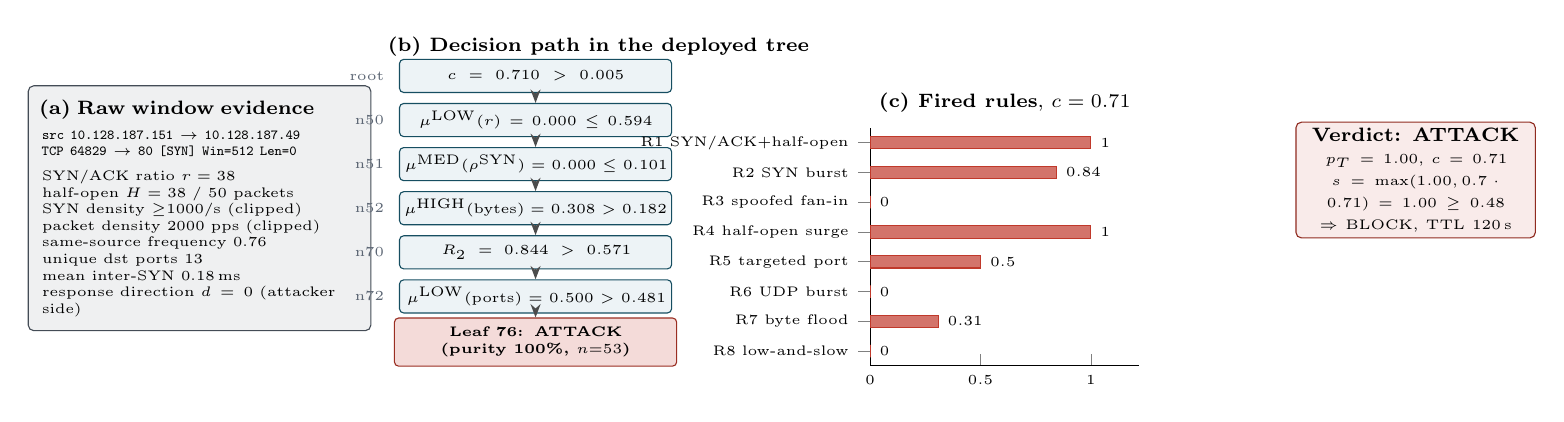
\begin{tikzpicture}[font=\scriptsize]
  % (a) raw evidence
  \node[box=gr, text width=4.0cm, align=left, anchor=west, font=\tiny, inner sep=5pt] (raw) at (0.3,-2.3) {%
   {\scriptsize\textbf{(a) Raw window evidence}}\\[3pt]
   {\tiny\ttfamily src 10.128.187.151 $\to$ 10.128.187.49}\\
   {\tiny\ttfamily TCP 64829 $\to$ 80 [SYN] Win=512 Len=0}\\[3pt]
   SYN/ACK ratio $r=38$\\
   half-open $H=38$ / 50 packets\\
   SYN density $\ge$1000/s (clipped)\\
   packet density 2000 pps (clipped)\\
   same-source frequency 0.76\\
   unique dst ports 13\\
   mean inter-SYN 0.18\,ms\\
   response direction $d=0$ (attacker side)};
  % (b) decision path
  \node[font=\scriptsize\bfseries, anchor=north west] at (4.75,0) {(b) Decision path in the deployed tree};
  \foreach \t/\v [count=\i from 0] in {
     {$c=0.710>0.005$}/root,
     {$\mu^{\mathrm{LOW}}(r)=0.000\le0.594$}/n50,
     {$\mu^{\mathrm{MED}}(\rho^{\mathrm{SYN}})=0.000\le0.101$}/n51,
     {$\mu^{\mathrm{HIGH}}(\text{bytes})=0.308>0.182$}/n52,
     {$R_2=0.844>0.571$}/n70,
     {$\mu^{\mathrm{LOW}}(\text{ports})=0.500>0.481$}/n72}{
     \node[draw=fz!70!black, fill=fz!8, rounded corners=1.5pt, text width=3.35cm, align=center, font=\tiny,
           minimum height=0.42cm, inner sep=1.5pt] (p\i) at (6.75,-0.62-\i*0.56) {\t};
     \node[font=\tiny, text=gr, anchor=east] at (4.95,-0.62-\i*0.56) {\v};
  }
  \node[draw=atk!80!black, fill=atk!18, rounded corners=1.5pt, text width=3.35cm, align=center, font=\tiny\bfseries,
        minimum height=0.48cm] (leaf) at (6.75,-4.0) {Leaf 76: ATTACK (purity 100\%, $n{=}53$)};
  \foreach \i [evaluate=\i as \j using int(\i+1)] in {0,...,4} \draw[arr] (p\i) -- (p\j);
  \draw[arr] (p5) -- (leaf);
  % (c) rule activations
  \begin{axis}[at={(11.0cm,-4.3cm)}, anchor=south west, width=5.0cm, height=4.6cm,
     xbar, bar width=4.5pt, xmin=0, xmax=1.22, y dir=reverse,
     symbolic y coords={R1,R2,R3,R4,R5,R6,R7,R8}, ytick=data,
     yticklabels={R1 SYN/ACK+half-open,R2 SYN burst,R3 spoofed fan-in,R4 half-open surge,R5 targeted port,R6 UDP burst,R7 byte flood,R8 low-and-slow},
     tick label style={font=\tiny}, title={\textbf{(c) Fired rules}, $c=0.71$}, title style={font=\scriptsize, yshift=-4pt},
     nodes near coords, nodes near coords style={font=\tiny, /pgf/number format/.cd, fixed, precision=2},
     axis x line*=bottom, axis y line*=left, xtick={0,0.5,1}, enlarge y limits=0.07]
     \addplot[fill=atk!70, draw=atk] coordinates {(1.0,R1) (0.844,R2) (0,R3) (1.0,R4) (0.5,R5) (0,R6) (0.308,R7) (0,R8)};
  \end{axis}
  % verdict
  \node[box=atk, text width=2.9cm, minimum height=1.0cm, anchor=north west] at (16.4,-1.2) {%
    \textbf{Verdict: ATTACK}\\{\tiny $p_T=1.00$, $c=0.71$}\\{\tiny $s=\max(1.00,0.7\cdot0.71)=1.00\ge0.48$}\\{\tiny $\Rightarrow$ BLOCK, TTL 120\,s}};
\end{tikzpicture}}
\caption{Anatomy of a real held-out verdict. (a) Transport-layer evidence of the window. (b) The six-condition path through the 89-node tree, ending in a pure attack leaf. (c) Activations of the eight direction-gated rules. The explanation is produced by the same fuzzy reasoning that produced the verdict; no post-hoc explainer is needed.}
\label{fig:case}
\end{figure*}

\subsection{From Manual Indicators to Automated Evidence}
Table~\ref{tab:mapping} maps each indicator used in the manual Wireshark investigations~\cite{naing2023,khaing2020} to its automated counterpart. Most indicators become continuous fuzzy evidence. ICMP-unreachable traffic is deliberately used as a \emph{direction cue} (victim-side control traffic) rather than as attack evidence. This keeps the victim's own error messages from being blamed on it.

\begin{table}[t]
\centering
\caption{Manual forensic indicators~\cite{naing2023,khaing2020} and their automated counterparts}
\label{tab:mapping}
\footnotesize
\renewcommand{\arraystretch}{1.1}
\setlength{\tabcolsep}{3pt}
\begin{tabular}{@{}>{\raggedright\arraybackslash}p{3.3cm} >{\raggedright\arraybackslash}p{4.7cm}@{}}
\toprule
\textbf{Manual indicator (Wireshark)} & \textbf{\fname{} counterpart} \\
\midrule
SYN vs.\ SYN-ACK counts (\texttt{tcp.flags} filters) & SYN/ACK ratio $r$, half-open $H$; rules R1, R3, R4 \\
I/O-graph spikes & SYN/packet/byte densities; R2, R4, R7 \\
Spoofed or repeated source IPs & same-source frequency $f$; R3 \\
Single targeted service port & dst-port diversity; R5 \\
UDP to port 80, UDP volume & UDP density, dst-port class; R6, R8 \\
ICMP host unreachable (\texttt{icmp.type==3}) & ICMP flag in direction gate $d$ \\
Packet-length bins (40--2,599\,B) & length mean / std.\ per window \\
Out-of-order, retransmissions & retransmission rate \\
Analyst's binary judgement & graded score $s$ + IF-THEN rule + action \\
\bottomrule
\end{tabular}
\end{table}

\subsection{Edge Feasibility}
On the Raspberry Pi the deployed path consists of pure-Python feature extraction ($\approx$1\,ms per window) followed by the fuzzy layer and the 89-node tree. During the live demonstration the dashboard telemetry showed about 23\% CPU, 41\% RAM and a SoC temperature of about 52\,$^\circ$C. In the scripted live scenarios, the \emph{congestion} phase (legitimate handshakes at a high rate) stayed in ALLOW because direction gating ignored the Pi's replies. During the \emph{SYN-flood} phase the score saturated at 1.0, the source was escalated to BLOCK, and the dashboard displayed the R1/R2 explanation (``high SYN burst paired with a low SYN-ACK ratio''). Blocked sources were released automatically after their TTL.

% =====================================================================
\section{Limitations and Threats to Validity}
\label{sec:limits}
\textbf{Single capture.} The results come from one lab capture with two attack phases (about 50\,s of flooding) from a single attacker host, against a large and diverse background. The spoofing option did not produce dispersed sources in the capture, so R3 was never exercised. Generalisation to other networks and to public benchmarks such as CICIoT2023~\cite{neto2023} and Bot-IoT~\cite{koroniotis2019} remains to be shown.
\textbf{Second flood phase.} Although the second phase was generated with the UDP-flood command, the attacker-to-victim packets labelled in it are TCP control traffic (RST/PSH-ACK). The static dataset's attack class is therefore TCP-centric. UDP-specific rules (R6, R8) were exercised only through the live simulator.
\textbf{Packet-level precision.} Precision is 34.5\% at packet granularity on a 13:1 imbalanced hold-out. Operationally, alerts are aggregated per source and per TTL, so one blocked host counts once. Window- or flow-level alerting would lower the alert volume further.
\textbf{Skewed attributes.} Percentile placement collapses to crisp steps for heavily skewed attributes. For example, the median UDP density in training is zero.
\textbf{Live features.} The retransmission feature relies on Wireshark annotations and is close to zero in live scapy mode. The live-edge observations are qualitative, and a systematic time-to-detect benchmark on the Pi is still pending.
\textbf{Induction method.} We use crisp CART over fuzzy features rather than native fuzzy-entropy ID3 with soft membership propagation.

% =====================================================================
\section{Conclusion and Future Work}
\label{sec:conclusion}
This paper presented \fname{}, which automates the transport-layer indicators of manual IoT network forensics~\cite{naing2023,khaing2020} with the fuzzy decision-tree reasoning proposed for forensic analysis~\cite{ye2022}, and deploys the result on a Raspberry Pi. Data-driven membership functions, eight direction-gated expert rules and a pruned decision tree trained only on the fuzzy space form a 9.1\,KB model. Under a leakage-free protocol it reaches 87.74\% accuracy and an F1 of 0.456. It beats an identically trained plain tree and a $125\times$ larger deep MLP, and raises 583 fewer false alarms than the plain tree. Every verdict carries a human-readable IF-THEN explanation and a graduated, reversible response. Equally important, we showed that weak labels (49.1\% victim replies) and random splits of rolling-window data can each distort IDS evaluation by several points, and we provided simple fixes for both.

Future work will (i) evaluate cross-dataset generalisation on CICIoT2023 and Bot-IoT and capture multi-host, genuinely spoofed and UDP-dominant floods; (ii) implement native Fuzzy-ID3 induction with fuzzy entropy and soft path propagation and compare it with the crisp-over-fuzzy tree; (iii) add the remaining indicators from the manual studies, namely TCP window-size anomaly (e.g., Win$=$256), Shannon source-IP entropy, ICMP-unreachable rate and a 100\,ms temporal burst score; (iv) estimate retransmissions from sequence numbers so the feature works in live mode; (v) adapt membership placement online with streaming quantiles; (vi) extend the rule base to application-layer IoT floods (HTTP, MQTT); and (vii) port inference to C/ONNX for microcontroller-class devices, together with a quantitative on-device time-to-detect benchmark.

\section*{Acknowledgment}
The authors thank the Indian Institute of Information Technology Sri City for the laboratory facilities and computing resources that supported this work.

% =====================================================================
\begin{thebibliography}{00}

\bibitem{naing2023} S. K. Naing, S. T. Oo, H. W. Y. Oo, P. Y. Lin, K. M. Nwe, and M. M. S. Thwin, ``IoT network forensics based on transport layer,'' in \emph{Proc. IEEE Conf. Comput. Appl. (ICCA)}, Yangon, Myanmar, Feb. 2023, pp. 312--317, doi: 10.1109/ICCA51723.2023.10182142.

\bibitem{antonakakis2017} M. Antonakakis \emph{et al.}, ``Understanding the Mirai botnet,'' in \emph{Proc. 26th USENIX Security Symp.}, Vancouver, BC, Canada, 2017, pp. 1093--1110.

\bibitem{kolias2017} C. Kolias, G. Kambourakis, A. Stavrou, and J. Voas, ``DDoS in the IoT: Mirai and other botnets,'' \emph{Computer}, vol. 50, no. 7, pp. 80--84, 2017.

\bibitem{eddy2007} W. Eddy, ``TCP SYN flooding attacks and common mitigations,'' IETF RFC 4987, Aug. 2007.

\bibitem{cert1996} CERT Coordination Center, ``TCP SYN flooding and IP spoofing attacks,'' CERT Advisory CA-1996-21, Carnegie Mellon Univ., Pittsburgh, PA, USA, 1996.

\bibitem{khaing2020} M. S. Khaing, Y. M. Thant, T. Tun, C. S. Htwe, and M. M. S. Thwin, ``IoT botnet detection mechanism based on UDP protocol,'' in \emph{Proc. IEEE Conf. Comput. Appl. (ICCA)}, Yangon, Myanmar, Feb. 2020.

\bibitem{stoyanova2020} M. Stoyanova, Y. Nikoloudakis, S. Panagiotakis, E. Pallis, and E. K. Markakis, ``A survey on the Internet of Things (IoT) forensics: Challenges, approaches, and open issues,'' \emph{IEEE Commun. Surveys Tuts.}, vol. 22, no. 2, pp. 1191--1221, 2nd Quart. 2020.

\bibitem{ye2022} J. Ye, ``A fuzzy decision tree reasoning method for network forensics analysis,'' in \emph{Proc. World Automation Congr. (WAC)}, San Antonio, TX, USA, Oct. 2022, pp. 41--45, doi: 10.23919/WAC55640.2022.9934389.

\bibitem{doshi2018} R. Doshi, N. Apthorpe, and N. Feamster, ``Machine learning DDoS detection for consumer Internet of Things devices,'' in \emph{Proc. IEEE Security Privacy Workshops (SPW)}, San Francisco, CA, USA, 2018, pp. 29--35.

\bibitem{meidan2018} Y. Meidan \emph{et al.}, ``N-BaIoT---Network-based detection of IoT botnet attacks using deep autoencoders,'' \emph{IEEE Pervasive Comput.}, vol. 17, no. 3, pp. 12--22, Jul.--Sep. 2018.

\bibitem{adadi2018} A. Adadi and M. Berrada, ``Peeking inside the black-box: A survey on explainable artificial intelligence (XAI),'' \emph{IEEE Access}, vol. 6, pp. 52138--52160, 2018.

\bibitem{bridges2000} S. M. Bridges and R. B. Vaughn, ``Fuzzy data mining and genetic algorithms applied to intrusion detection,'' in \emph{Proc. 23rd Nat. Inf. Syst. Security Conf. (NISSC)}, Baltimore, MD, USA, 2000.

\bibitem{koroniotis2019} N. Koroniotis, N. Moustafa, E. Sitnikova, and B. Turnbull, ``Towards the development of realistic botnet dataset in the Internet of Things for network forensic analytics: Bot-IoT dataset,'' \emph{Future Gener. Comput. Syst.}, vol. 100, pp. 779--796, 2019.

\bibitem{zadeh1965} L. A. Zadeh, ``Fuzzy sets,'' \emph{Inf. Control}, vol. 8, no. 3, pp. 338--353, 1965.

\bibitem{quinlan1986} J. R. Quinlan, ``Induction of decision trees,'' \emph{Mach. Learn.}, vol. 1, no. 1, pp. 81--106, 1986.

\bibitem{breiman1984} L. Breiman, J. H. Friedman, R. A. Olshen, and C. J. Stone, \emph{Classification and Regression Trees}. Belmont, CA, USA: Wadsworth, 1984.

\bibitem{yuan1995} Y. Yuan and M. J. Shaw, ``Induction of fuzzy decision trees,'' \emph{Fuzzy Sets Syst.}, vol. 69, no. 2, pp. 125--139, 1995.

\bibitem{janikow1998} C. Z. Janikow, ``Fuzzy decision trees: Issues and methods,'' \emph{IEEE Trans. Syst., Man, Cybern. B, Cybern.}, vol. 28, no. 1, pp. 1--14, Feb. 1998.

\bibitem{dimolianis2021} A. Dimolianis, A. Pavlidis, and V. Maglaris, ``SYN flood attack detection and mitigation using machine learning traffic classification and programmable data plane filtering,'' in \emph{Proc. 24th Conf. Innov. Clouds, Internet Netw. Workshops (ICIN)}, Paris, France, 2021, pp. 126--133.

\bibitem{hoang2022} T.-M. Hoang, N.-H. Tran, V.-L. Thai, D.-L. Nguyen, and N.-H. Nguyen, ``An efficient IDS using FIS to detect DDoS in IoT networks,'' in \emph{Proc. 9th NAFOSTED Conf. Inf. Comput. Sci. (NICS)}, 2022.

\bibitem{keshavamurthy2024} P. Keshavamurthy and S. Kulkarni, ``A hybrid machine learning--fuzzy cognitive map approach for fast, reliable DDoS attack detection,'' in \emph{Proc. Cyber Secur. Netw. Conf. (CSNet)}, 2024, pp. 228--235, doi: 10.1109/CSNET64211.2024.10851754.

\bibitem{kim2024} C. Kim, C. So-In, Y. Kongsorot, and P. Aimtongkham, ``FLSec-RPL: A fuzzy logic-based intrusion detection scheme for securing RPL-based IoT networks against DIO neighbor suppression attacks,'' \emph{Cybersecurity}, vol. 7, 2024, doi: 10.1186/s42400-024-00223-x.

\bibitem{neto2023} E. C. P. Neto, S. Dadkhah, R. Ferreira, A. Zohourian, R. Lu, and A. A. Ghorbani, ``CICIoT2023: A real-time dataset and benchmark for large-scale attacks in IoT environment,'' \emph{Sensors}, vol. 23, no. 13, Art. no. 5941, 2023.

\bibitem{hping3} S. Sanfilippo, ``hping3: Active network security tool,'' [Online]. Available: \url{http://www.hping.org}

\bibitem{scapy} P. Biondi and the Scapy community, ``Scapy: Packet manipulation program and library,'' [Online]. Available: \url{https://scapy.net}

\bibitem{breiman2001} L. Breiman, ``Random forests,'' \emph{Mach. Learn.}, vol. 45, no. 1, pp. 5--32, 2001.

\bibitem{pedregosa2011} F. Pedregosa \emph{et al.}, ``Scikit-learn: Machine learning in Python,'' \emph{J. Mach. Learn. Res.}, vol. 12, pp. 2825--2830, 2011.

\end{thebibliography}

\end{document}
